%\chapter{Risultati numerici}
\section{Risultati numerici}
\label{chap:Results}
In questo capitolo verranno esposti i risultati numerici ottenuti.
I due esempi utilizzati come casi test sono stati presi da \cite{MAIN}.
In entrambi questi esempi verrà considerato l'operatore lineare affine $\tilde{B}$ \eqref{eq:210}.
\par
Si considera come dominio spaziale il quadrato $ \Omega = (0,1)^2$ ed una mesh uniforme definita da
\begin{Code}[caption={mesh in spazio square( 150, 150, flags=1 )}]
-- Square mesh : nb vertices  = 22801 ,  nb triangles = 45000 ,  nb boundary edges 600
\end{Code}

\subsection{Test Case 01}
\subsubsection{Set-up}
Il primo esempio considerato è in accordo con l'ipotesi i) introdotta nella sezione \ref{chap:Continuos}.
Preso il dominio spazio-temporale $\Omega \times I = (0,1)^2 \times (0,0.01)$ e d=1, si considera l'operatore di controllo lineare affine $\tilde{B}$ che può essere completamente caratterizzato da:
{\renewcommand\arraystretch{2}
\begin{equation}
\begin{array}{c}
g_1(x_1,x_2) = sin({\pi}x_1)sin({\pi}x_2)\\
g_0(t,x_1,x_2) = -{\pi}^2w_a(t,x_1,x_2) - BP_{U_{ad}} \left( -\frac{1}{4\alpha}(exp(a{\pi}^2t)-exp(a{\pi}^2T)) \right)
\end{array}
\label{eq:500}
\end{equation}
}
dove
\begin{equation}
w_a(t,x_1,x_2) = exp(a{\pi}^2t)sin({\pi}x_1)sin({\pi}x_2) \text{, } a \in \mathbb{R}
\label{eq:501}
\end{equation}
In particolare vengono considerate le costanti $a=-\sqrt{5}$ ed $\alpha={\pi}^{-4}$.
Come conseguenza di ciò si ha che \eqref{eq:212} verrà riscritta, utilizzando l'aggiunto di B e non $\tilde{B}$, come:
\begin{equation}
(B'z)(t) = \int_{\Omega} z(t,x_1,x_2)g_1(x_1,x_2) ,dx_1dx_2
\label{eq:502}
\end{equation}
Si definiscono ora:
{\renewcommand\arraystretch{2}
\begin{equation}
\begin{array}{c}
y_d(t,x_1,x_2) = \frac{a^2 - 5}{2 + a}{\pi}^2w_a(t,x_1,x_2) + 2{\pi}^2w_a(T,x_1,x_2) \\
y_0(x_1,x_2) = \frac{- 1}{2 + a}{\pi}^2w_a(0,x_1,x_2)
\end{array}
\label{eq:503}
\end{equation}
}
L'insieme ammissibile $U_{ad}$ è limitato inferiormente da $a_1=-25$ e superiormente da $b_1=-1$.
Infine definiamo le soluzioni esatte per il problema di controllo ottimo \ref{eq:200}:
{\renewcommand\arraystretch{2}
\begin{equation}
\begin{array}{c}
\overline{u}(t,x_1,x_2) = P_{U_{ad}} \left( -\frac{1}{4\alpha}(\exp(a{\pi}^2t)-\exp(a{\pi}^2T)) \right) \\
\overline{y}(t,x_1,x_2) = \frac{- 1}{2 + a}{\pi}^2w_a(0,x_1,x_2) \\
\overline{p}(t,x_1,x_2) = w_a(t,x_1,x_2) - w_a(T,x_1,x_2)
\end{array}
\label{eq:504}
\end{equation}
}

\subsubsection{Risultati Numerici}
La tabelle \ref{puntofissoI}, \ref{puntofissoIbis}, \ref{newtonI} e \ref{newtonIbis} mostrano il comportamento degli errori considerati e il valore dell'ordine di convergenza per diverse griglie temporali. Si può notare che sia per l'algoritmo di punto fisso che quello di semi-Newton l'andamento dell'errore \ref{eq:errcon} è di $O(k^2)$ in accordo col risultato teorico \ref{controlteo} e con i risultati numerici di \cite{MAIN}. In particolare si rileva che l'ordine di convergenza diminuisce per l'ultimo livello in cui la griglia temporale non è più indipendente da quella spaziale. Essendo la variabile di stato costante a tratti nel tempo l'ordne di convergenza riscontrato è solo uno, ma un ordine due è ottenuto per la proiezione della variabile di stato $\pi_{{P^*}_k}y_k$ conformemente con il \textbf{Lemma} \ref{conv:stato}.

\begin{table}
\caption{Punto fisso per Test case 01: errori e EOC }
\label{puntofissoI}
\centering

\begin{tabular}{cllll}
\toprule
{l}           &  {$ \norma{\bar{u}-u_{kh}}_{L^2(L^2)} $} &  {$ \norma{\bar{y}-y_{kh}}_{L^2(L^2)} $} &  {$ EOC_u $} &  {$ EOC_y $} \\
\midrule
1            &  0.31667 &  0.981285 &  {$-$} &  {$-$} \\
2            &  0.0835064 &  0.496296 &  2.60937 &  1.33449 \\
3            &  0.0209608 &  0.248822 &  2.35165 &  1.17464 \\
4            &  0.00500916 &  0.124494 &  2.25065 &  1.08882 \\
5            &  0.00109219  &  0.0622586 &  2.29624 &  1.04473 \\
6            &  0.000497644 &  0.0311327 &  1.15957 &  1.02236 \\
\bottomrule
\end{tabular}              

\end{table}


\begin{table}
\caption{Punto fisso per Test case 01: errori e EOC }
\label{puntofissoIbis}
\centering

\begin{tabular}{cllll}
\toprule
{l}           &  {$ \norma{\bar{y}-\pi_{P^*_k}y_{kh}}_{L^2(L^2)} $} &  {$ \norma{\bar{p}-p_{kh}}_{L^2(L^2)} $} &  {$ EOC_{\pi y} $} &  {$ EOC_p $} \\
\midrule
1            &  0.520894 &  0.00660747 &  {$-$} &  {$-$} \\
2            &  0.15134 &  0.00173155 &  2.41965 &  2.6216 \\
3            &  0.0393476 &  0.00043334 &  2.29181 &  2.35673 \\
4            &  0.00970087 &  0.000103613 &  2.20164 &  2.24982 \\
5            &  0.00221619 &  0.000022824 &  2.2259 &  2.28078 \\
6            &  0.000432024 &  0.000010724 &  2.41203 &  1.11429 \\
\bottomrule
\end{tabular}              

\end{table}
\begin{figure}
\centering
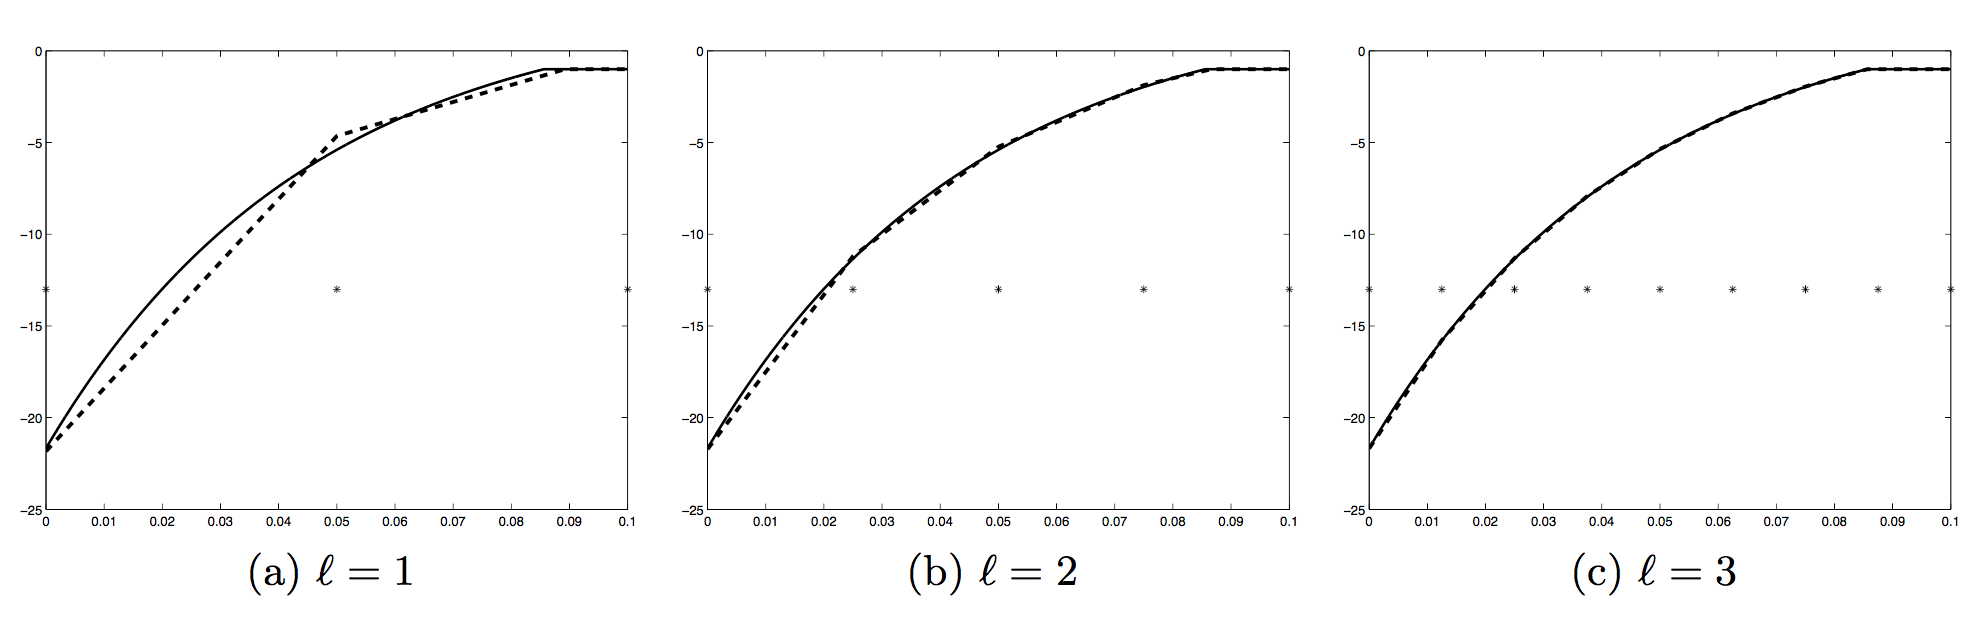
\includegraphics[width=\linewidth]{img/cap6/TestCase01_ues_paper}
\caption{Test Case 01 $\overline{u}$ e $u_k$ risultati di \cite{MAIN}}
\label{fig:500}
\end{figure}

\begin{figure}
\centering%
\subfigure[\protect\url{l = 1}]%
{\includegraphics[width=0.3\linewidth]{img/cap6/Imm_PF_01/ControlSol_N150_l1}}\qquad
\subfigure[\protect\url{l = 2}]%
{\includegraphics[width=0.3\linewidth]{img/cap6/Imm_PF_01/ControlSol_N150_l2}}\qquad
\subfigure[\protect\url{l = 3}]%
{\includegraphics[width=0.3\linewidth]{img/cap6/Imm_PF_01/ControlSol_N150_l3}}\qquad
\subfigure[\protect\url{l = 4}]%
{\includegraphics[width=0.3\linewidth]{img/cap6/Imm_PF_01/ControlSol_N150_l4}}\qquad
\subfigure[\protect\url{l = 5}]%
{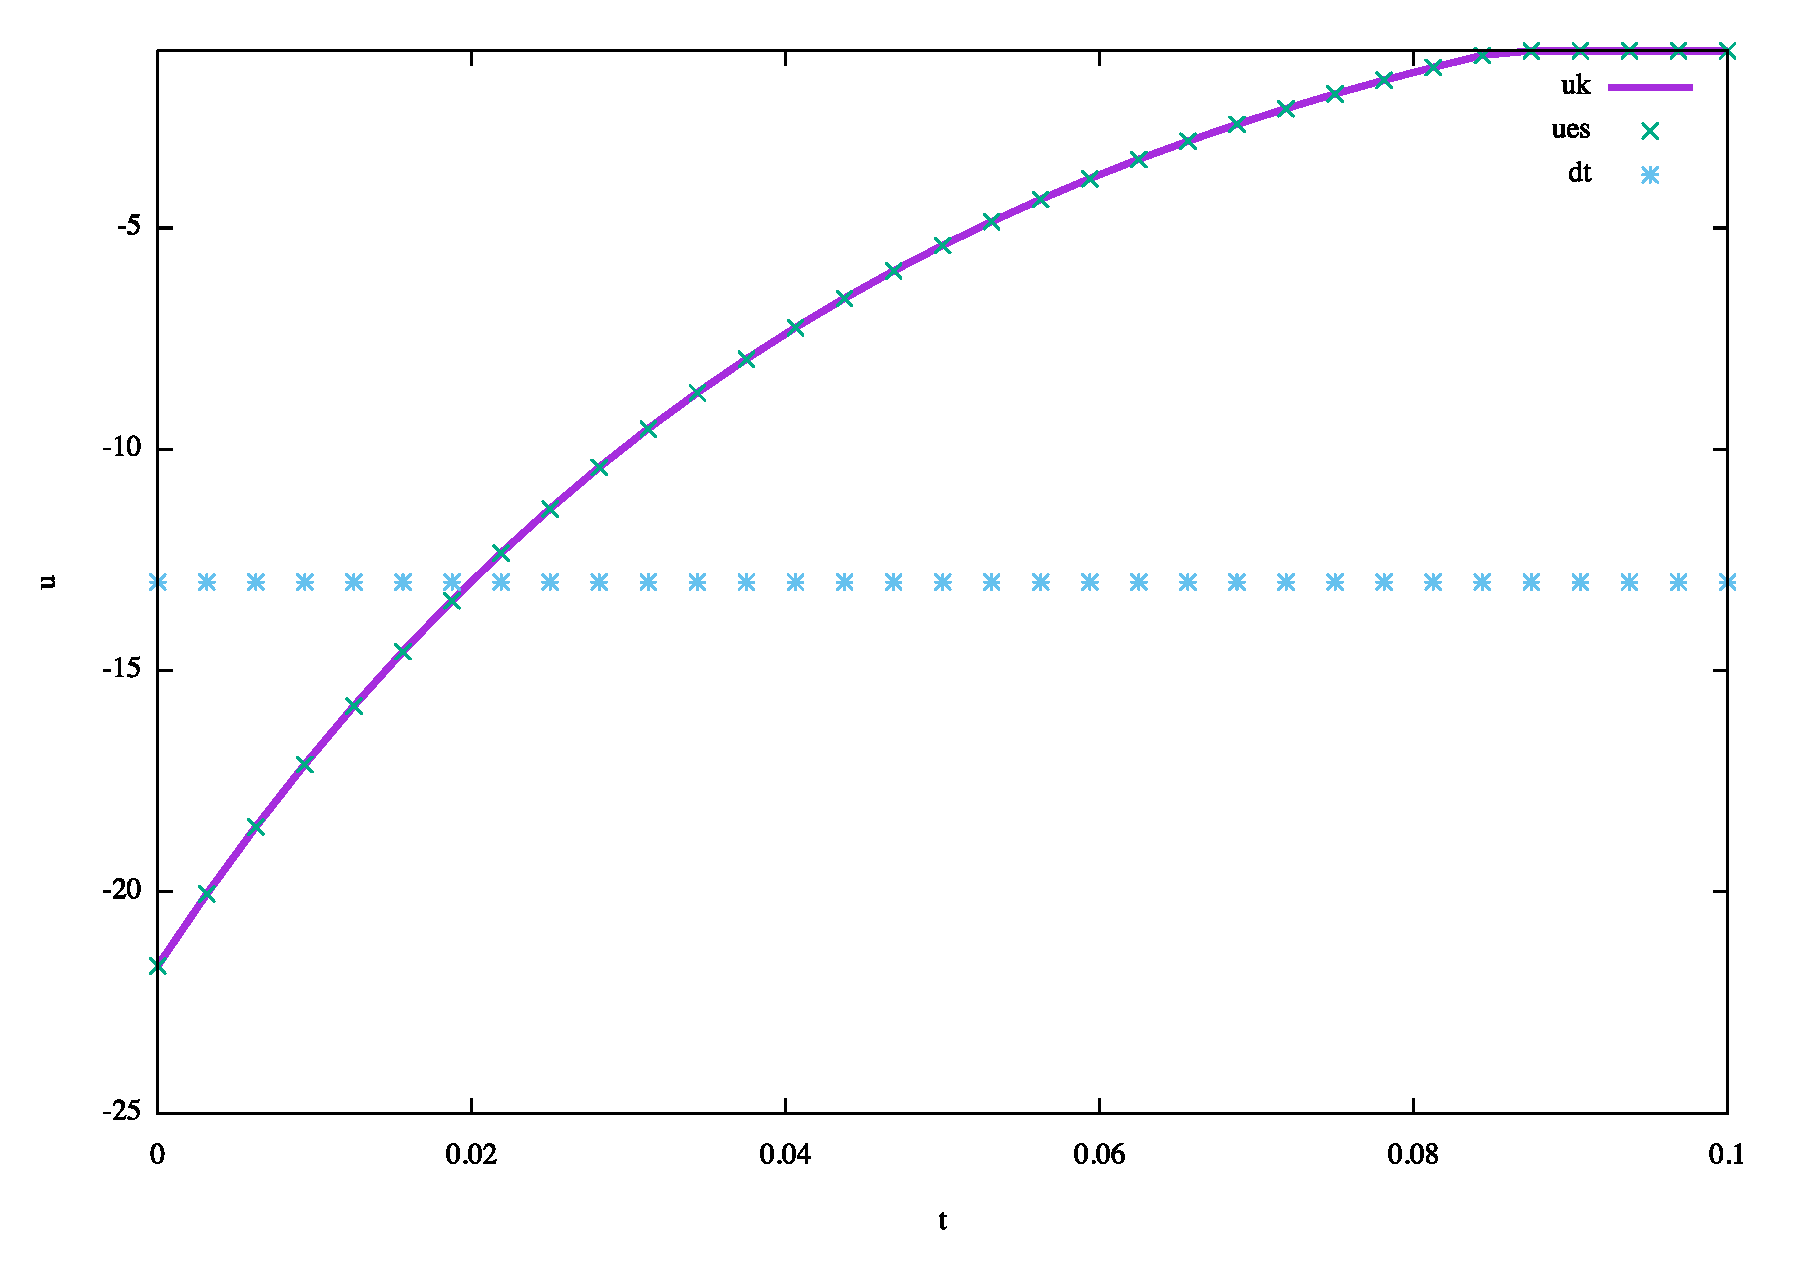
\includegraphics[width=0.3\linewidth]{img/cap6/Imm_PF_01/ControlSol_N150_l5}}\qquad
\subfigure[\protect\url{l = 6}]%
{\includegraphics[width=0.3\linewidth]{img/cap6/Imm_PF_01/ControlSol_N150_l6}}
\caption{Test Case 01 $\overline{u}$ e $u_k$ risultati dell'algoritmo di punto fisso}
\label{fig:501}
\end{figure}

\begin{table}
\caption{Newton per Test case 01: errori e EOC }
\label{newtonI}
\centering

\begin{tabular}{cllll}
\toprule
{l}           &  {$ \norma{\bar{u}-u_{kh}}_{L^2(L^2)} $} &  {$ \norma{\bar{y}-y_{kh}}_{L^2(L^2)} $} &  {$ EOC_u $} &  {$ EOC_y $} \\
\midrule
1            &  0.316669 &  0.981285 &  {$-$} &  {$-$} \\
2            &  0.0835064 &  0.496296 &  2.60937 &  1.33449 \\
3            &  0.0209612 &  0.248822 &  2.35161 &  1.17464 \\
4            &  0.00500971 &  0.124494  &  2.25051 &  1.08882 \\
5            &  0.00109312 &  0.0622586 &  2.29512 &  1.04473 \\
6            &  0.000497833 &  0.0311327 &  1.16028 &  1.02236 \\
\bottomrule
\end{tabular}              

\end{table}


\begin{table}
\caption{Newton per Test case 01: errori e EOC }
\label{newtonIbis}
\centering

\begin{tabular}{cllll}
\toprule
{l}           &  {$ \norma{\bar{y}-\pi_{P^*_k}y_{kh}}_{L^2(L^2)} $} & {$ \norma{\bar{p}-p_{kh}}_{L^2(L^2)} $} &  {$ EOC_{\pi y} $}  &  {$ EOC_p $} \\
\midrule
1            &  0.520894 &  0.00660747 &  {$-$} &  {$-$} \\
2            &  0.15134 &  0.00173155 &  2.41965 &  2.6216 \\
3            &  0.0393476 &  0.00043334 &  2.29181 &  2.35672 \\
4            &  0.00970089 &  0.000103614 &  2.20164 &  2.24981 \\
5            &  0.00221621 &  0.0000228246 &  2.22589 &  2.28078 \\
6            &  0.000432023 &  0.0000107235 &  2.41204 &  1.11436 \\
\bottomrule
\end{tabular}              

\end{table}

\begin{figure}
\centering%
\subfigure[\protect\url{l = 1}]%
{\includegraphics[width=0.3\linewidth]{img/cap6/Imm_CG_01/ControlSol_N150_l1}}\qquad
\subfigure[\protect\url{l = 2}]%
{\includegraphics[width=0.3\linewidth]{img/cap6/Imm_CG_01/ControlSol_N150_l2}}\qquad
\subfigure[\protect\url{l = 3}]%
{\includegraphics[width=0.3\linewidth]{img/cap6/Imm_CG_01/ControlSol_N150_l3}}\qquad
\subfigure[\protect\url{l = 4}]%
{\includegraphics[width=0.3\linewidth]{img/cap6/Imm_CG_01/ControlSol_N150_l4}}\qquad
\subfigure[\protect\url{l = 5}]%
{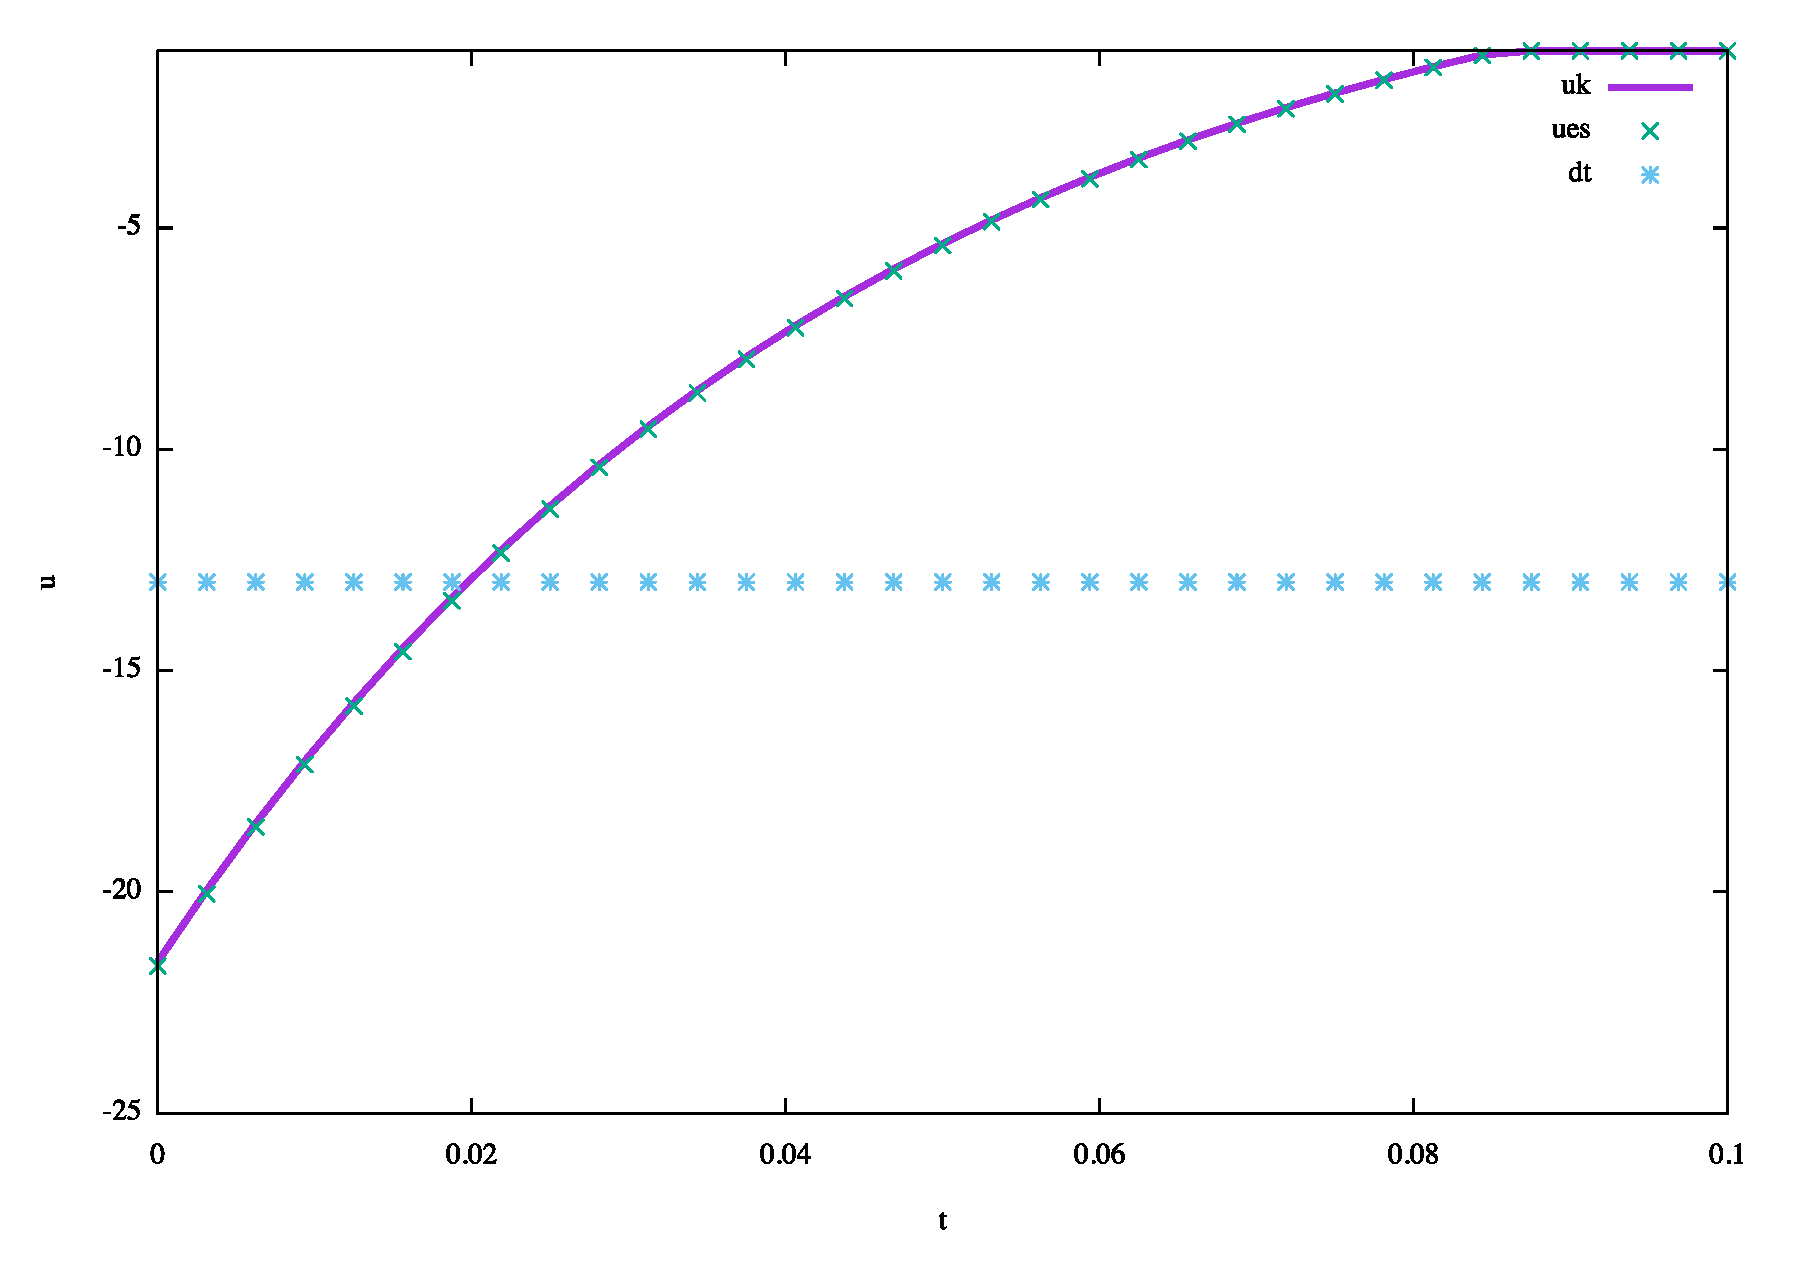
\includegraphics[width=0.3\linewidth]{img/cap6/Imm_CG_01/ControlSol_N150_l5}}\qquad
\subfigure[\protect\url{l = 6}]%
{\includegraphics[width=0.3\linewidth]{img/cap6/Imm_CG_01/ControlSol_N150_l6}}
\caption{Test Case 01 $\overline{u}$ e $u_k$: risultati dell'algortimo semi Newton}
\label{fig:502}
\end{figure}

In figura \ref{eq:500} sono riportati i risultati del paper \cite{MAIN} nei primi tre livelli di raffinamento di griglia. Mentre in \ref{eq:501} e \ref{eq:502} quelli ottenuti con il codice implementato per questo lavoro per ogni livello considerato. In entrambi i casi si vede che una buona approssimazione della soluzione esatta viene raggiunta.
\par
Per l'algoritmo di punto fisso sono richieste cinque o sei iterazioni per ogni griglia temporale prima di arrivare a convergenza, considerando un valore di tolleranza di $toll=10^{-5}$. Mentre per quello di Newton ne bastano quattro. 

\subsection{Test Case 02}
\subsubsection{Set-up}
Il secondo esempio considerato è in accordo con l'ipotesi i) introdotta in \ref{chap:Continuos}.
Preso il dominio spazio-temporale $\Omega \times I = (0,1)^2 \times (0,0.5)$ e d=1, si considera l'operatore di controllo lineare affine $\tilde{B}$ che può essere completamente caratterizzato da:
{\renewcommand\arraystretch{2}
\begin{equation}
\begin{array}{c}
g_1(x_1,x_2) = sin({\pi}x_1)sin({\pi}x_2)\\
g_0(t,x_1,x_2) = g_1(x_1,x_2) 2\pi \left( -\frac{a}{T}sin\left( \frac{t}{T}2{\pi}a \right) + \pi cos\left( \frac{t}{T}2{\pi}a \right) \right) - B\overline{u}
\end{array}
\label{eq:505}
\end{equation}
}
In particolare vengono considerate le costanti $a=-2$ ed $\alpha=1$.
Si definiscono ora:
{\renewcommand\arraystretch{2}
\begin{equation}
\begin{array}{c}
y_d(t,x_1,x_2) = g_1\left( cos\left( \frac{t}{T}2{\pi}a \right)(1-2{\pi}^2) -\frac{2{\pi}a}{T}sin\left( \frac{t}{T}2{\pi}a \right) +2{\pi}^2cos(2{\pi}a) \right)\\
y_0(x_1,x_2) = g_1(x_1,x_2)
\end{array}
\label{eq:506}
\end{equation}
}
L'insieme ammissibile $U_{ad}$ è limitato inferiormente da $a_1=0.2$ e superiormente da $b_1=0.4$.
Infine definiamo le soluzioni esatte per il problema di controllo ottimo \ref{eq:200}:
{\renewcommand\arraystretch{2}
\begin{equation}
\begin{array}{c}
\overline{u}(t,x_1,x_2) = P_{U_{ad}} \left( -\frac{1}{4\alpha}cos \left( \frac{t}{T}2{\pi}a \right) +\frac{1}{4\alpha} \right) \\
\overline{y}(t,x_1,x_2) = \frac{- 1}{2 + a}{\pi}^2w_a(0,x_1,x_2) \\
\overline{p}(t,x_1,x_2) = w_a(t,x_1,x_2) - w_a(T,x_1,x_2)
\end{array}
\label{eq:507}
\end{equation}
}
dove
\begin{equation}
w_a(t,x_1,x_2) = cos \left( \frac{t}{T}2{\pi}a \right) \cdot g_1(t,x_1,x_2)
\label{eq:508}
\end{equation}

\subsubsection{Risultati Numerici}
I risultati per gli errori di convergenza sono gli stessi tratti per il caso 01 e rispecchiano quelli esposti in \cite{MAIN}. Essendo la soluzione esatta $\overline{u}$ più complessa in questo test case, si nota che i primi due livelli di griglia non danno risultati rappresentativi. Infatti il numero di punti di non derivabilità della $\overline{u}$ è maggiore dei nodi della griglia temporale considerata.
La perdita riscontrata nell'ordine di convergenza per l'ultima mesh temporale è invece da attribuire all'influenza dell'errore in spazio.
\par
In figura \ref{eq:503} sono riportati i risultati del paper \cite{MAIN} nei primi tre livelli di raffinamento di griglia. Mentre in \ref{eq:504} e \ref{eq:505} quelli ottenuti con il codice implementato per questo lavoro per ogni livello considerato. In entrambi i casi si vede che una buona approssimazione della soluzione esatta viene raggiunta.
\par
Per l'algoritmo di punto fisso sono richieste due iterazioni per ogni griglia temporale prima di arrivare a convergenza, considerando un valore di tolleranza di $toll=10^{-5}$, mentre per quello di Newton ne bastano tre se viene introdotto un criterio di tolleranza aggiuntivo tale per cui:
\begin{equation}
\norma{\nabla\phi(w^k)} - \norma{\nabla\phi(w^{k+1}} > t_0
\label{primanorma}
\end{equation} 
oppure quattro se viene considerato invece:
\begin{equation}
\norma{\nabla\phi(w^k) - \nabla\phi(w^{k+1}} > t_0
\label{secondanorma}
\end{equation}
Col criterio \ref{primanorma} l'algoritmo converge in tre passi per ognuna delle mesh considerate. Mentre utilizzando \ref{secondanorma} si ha la convergenza dopo nove passi per la prima griglia utilizzata e quattro dalla successiva in avanti.

\begin{figure}
\centering
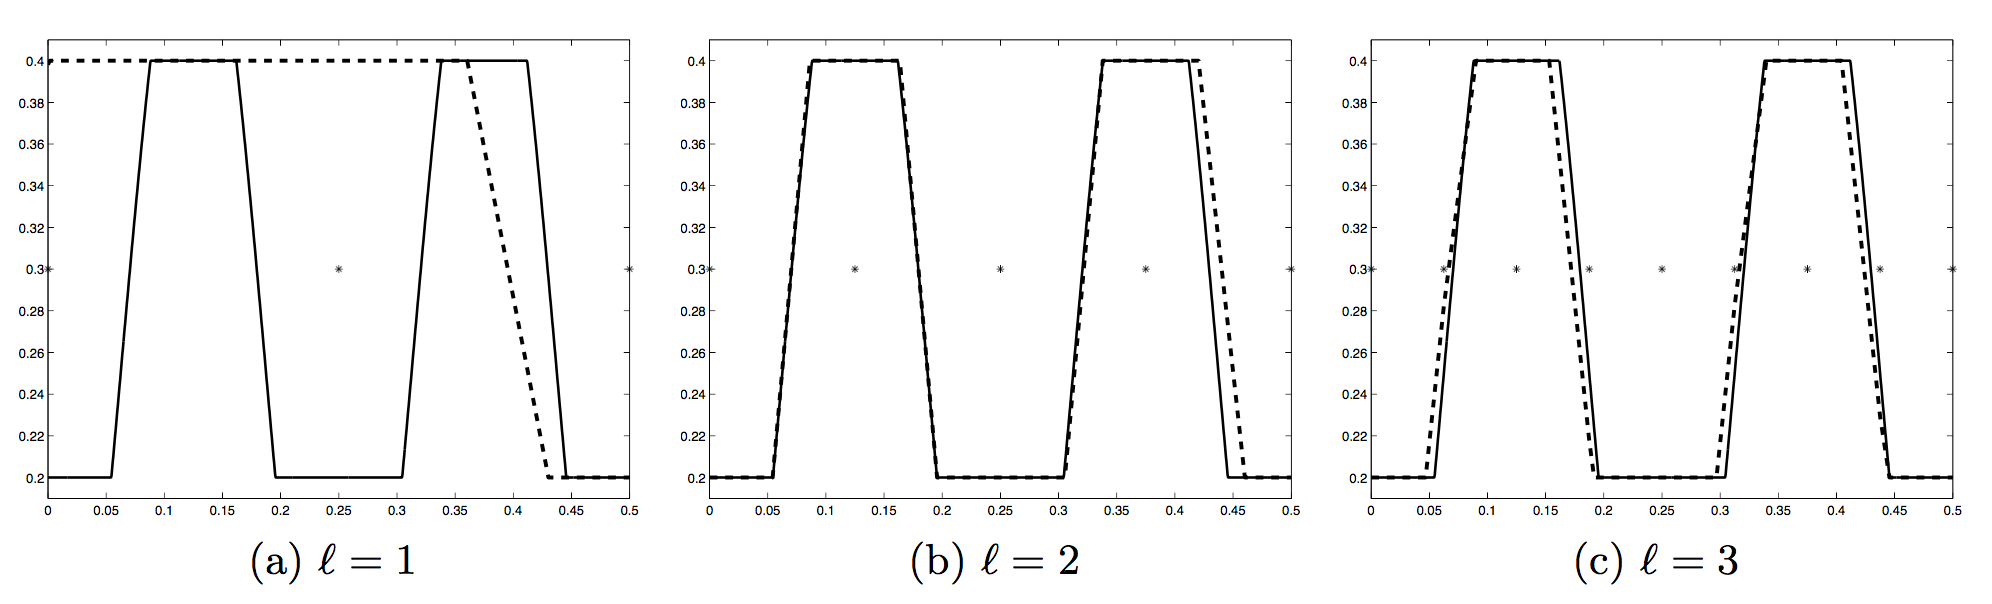
\includegraphics[width=\linewidth]{img/cap6/TestCase02_ues_paper}
\caption{Test Case 02 $\overline{u}$ e $u_k$ risultati di \cite{MAIN}}
\label{fig:503}
\end{figure}

\begin{table}
\caption{Punto fisso per Test case II: errori e EOC }
\label{puntofissoII}
\centering

\begin{tabular}{cllll}
\toprule
{l}           &  {$ \norma{\bar{u}-u_{kh}}_{L^2(L^2)} $} &  {$ \norma{\bar{y}-y_{kh}}_{L^2(L^2)} $} &  {$ EOC_{u} $} &  {$ EOC_y $} \\
\midrule
1            &  0.11547 &  0.577323 &  {$-$} &  {$-$} \\
2            &  0.049267 &  0.463462 &  1.66741 &  0.430045 \\
3            &  0.0229418 &  0.136413 &  1.30029 &  2.08074 \\
4            &  0.0036817 &  0.0594452 &  2.87676 &  1.30605 \\
5            &  0.000908002 &  0.0286805 &  2.1105 &  1.09882 \\
6            &  0.000229782  &  0.0142118 &  2.02708 &  1.0358 \\
7            &  0.0000652737 &  0.0070899 &  1.83615 &  1.01455 \\      
8            &  0.0000267529 &  0.003543 &  1.29406 &  1.00643 \\
\bottomrule
\end{tabular}              

\end{table}


\begin{table}
\caption{Punto fisso per Test case II: errori e EOC }
\label{puntofissoIIbis}
\centering

\begin{tabular}{cllll}
\toprule
{l}           &  {$ \norma{\bar{y}-\pi_{P^*_k}y_{kh}}_{L^2(L^2)} $} &  {$ \norma{\bar{p}-p_{kh}}_{L^2(L^2)} $} &  {$ EOC_{\pi y} $} &  {$ EOC_p $} \\
\midrule
1            &  0.408219 &  0.57735 &  {$-$} &  {$-$} \\
2            &  0.428289 &  0.181146 &  0.0939571 &  2.26916 \\
3            &  0.108057  &  0.0846821 &  2.34293 &  1.29366 \\
4            &  0.0223162  &  0.0224906 &  2.48014 &  2.08464 \\
5            &  0.00443799 &  0.00571816 &  2.43498 &  2.06462 \\
6            &  0.000929298 &  0.00145281 &  2.3065 &  2.02122 \\
7            &  0.000203934 &  0.000385864 &  2.21269 &  1.93423 \\      
8            &  0.0000465654 &  0.000130114 &  2.14277 &  1.57715 \\
\bottomrule
\end{tabular}              

\end{table}

\begin{figure}
\centering%
\subfigure[\protect\url{l = 1}]%
{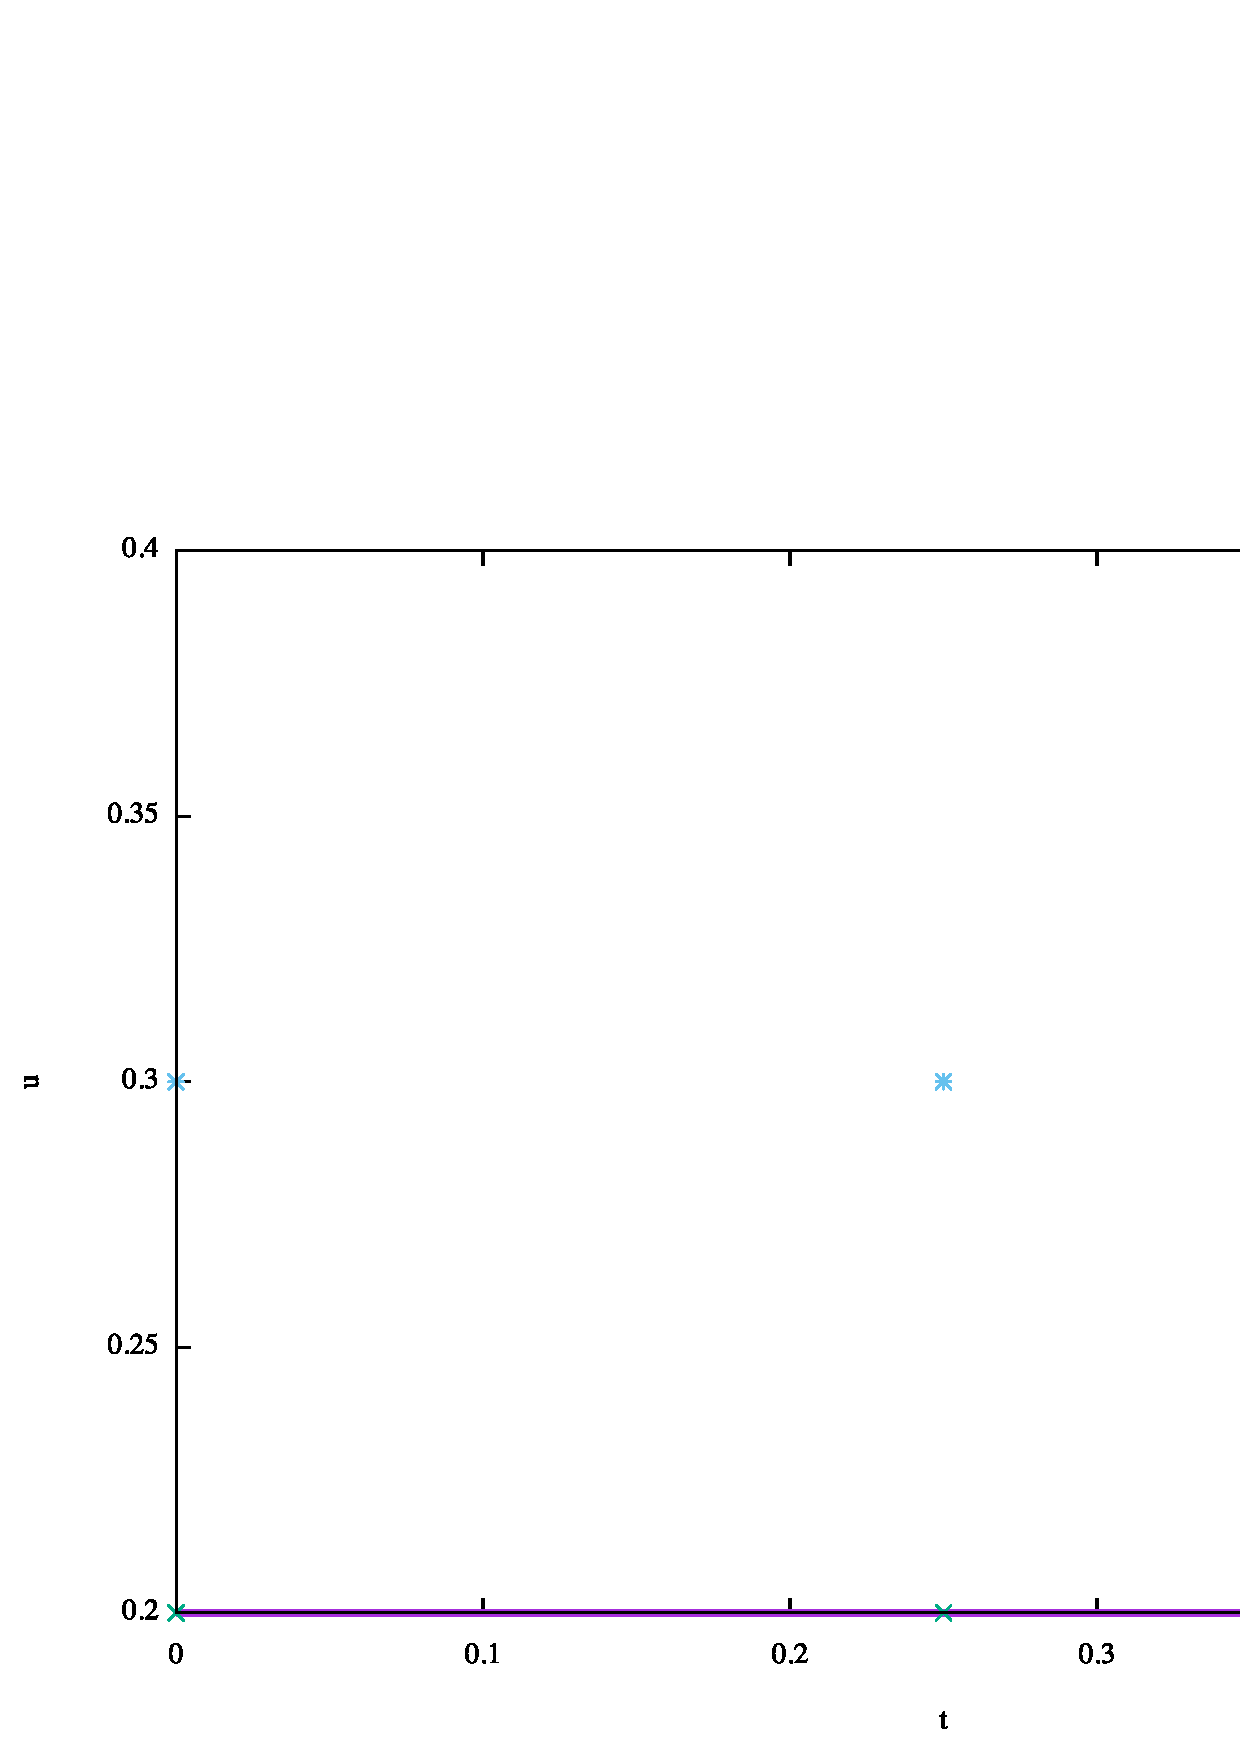
\includegraphics[width=0.3\linewidth]{img/cap6/Imm_PF_02/ControlSol_N150_l1}}\qquad
\subfigure[\protect\url{l = 2}]%
{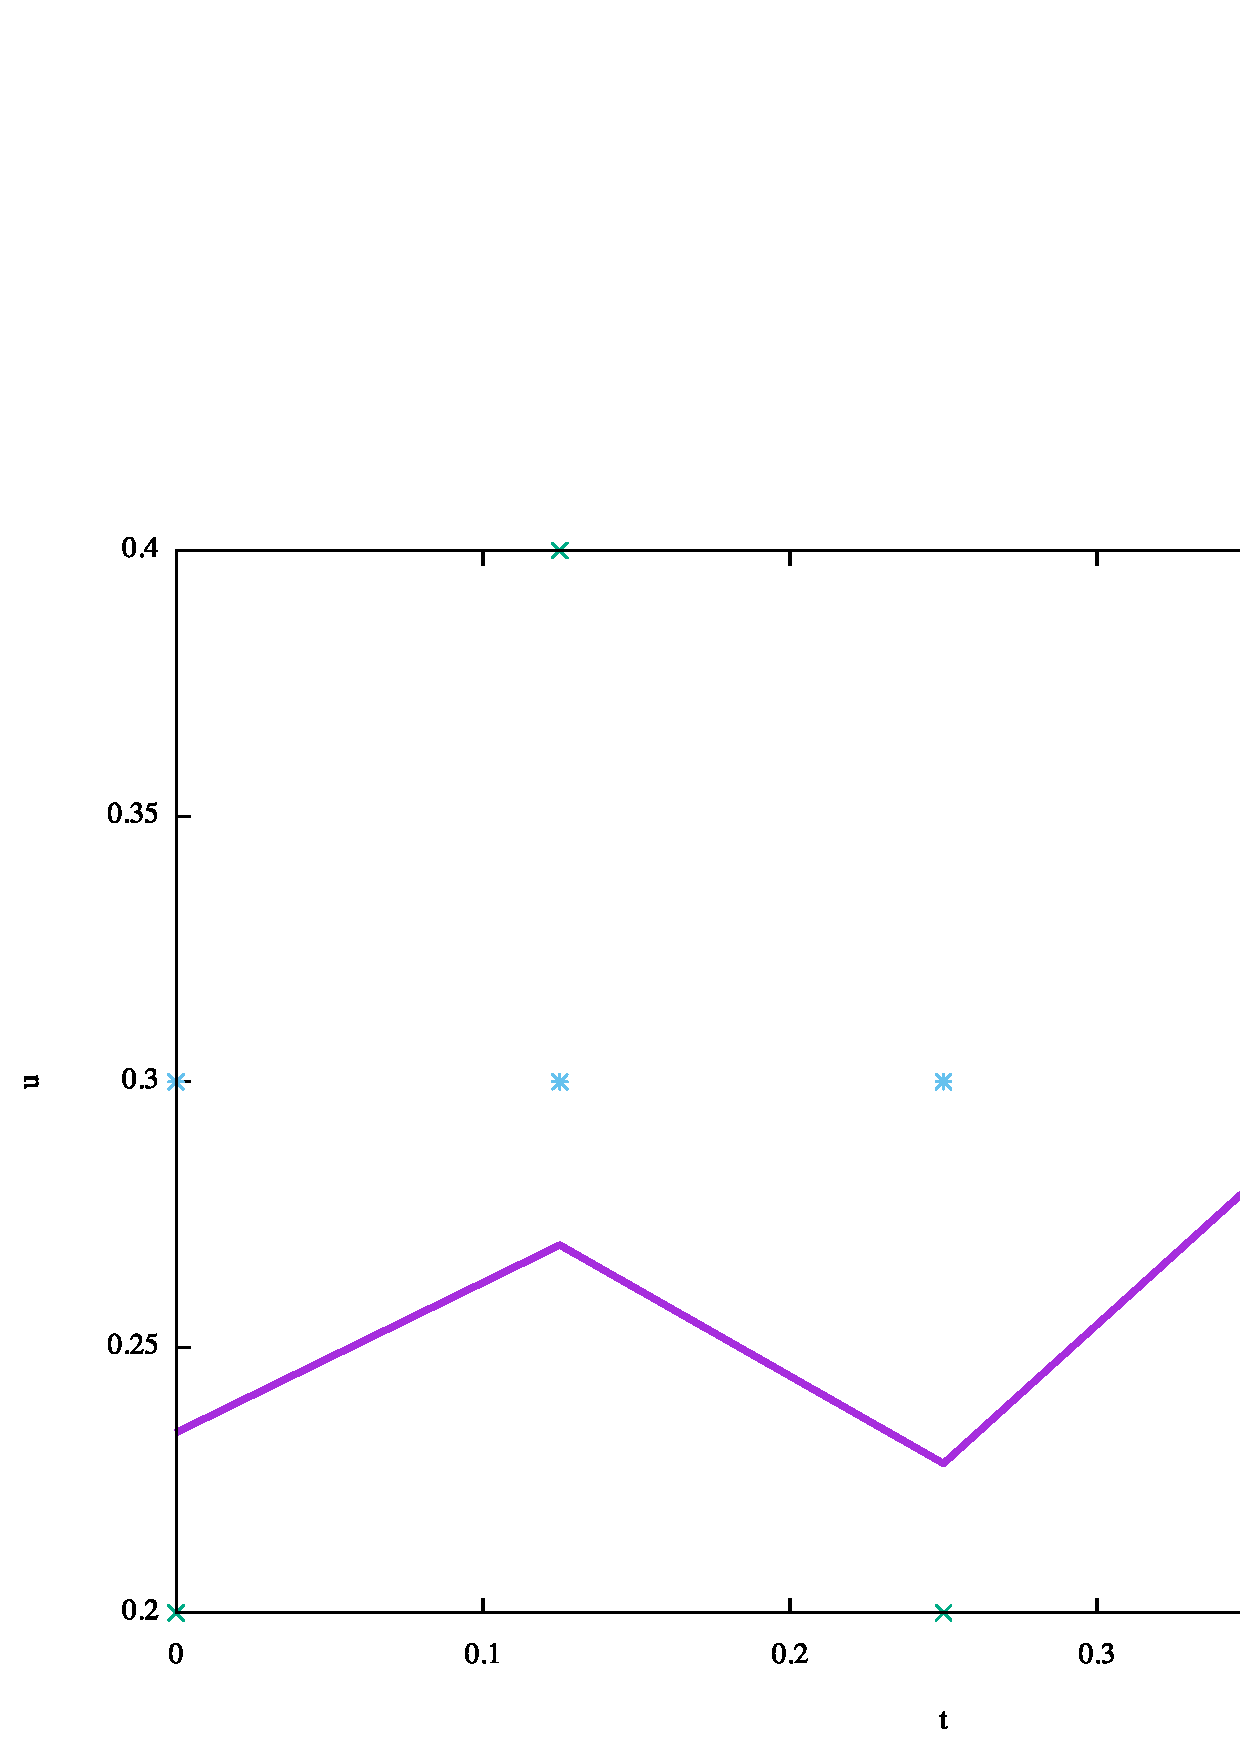
\includegraphics[width=0.3\linewidth]{img/cap6/Imm_PF_02/ControlSol_N150_l2}}\qquad
\subfigure[\protect\url{l = 3}]%
{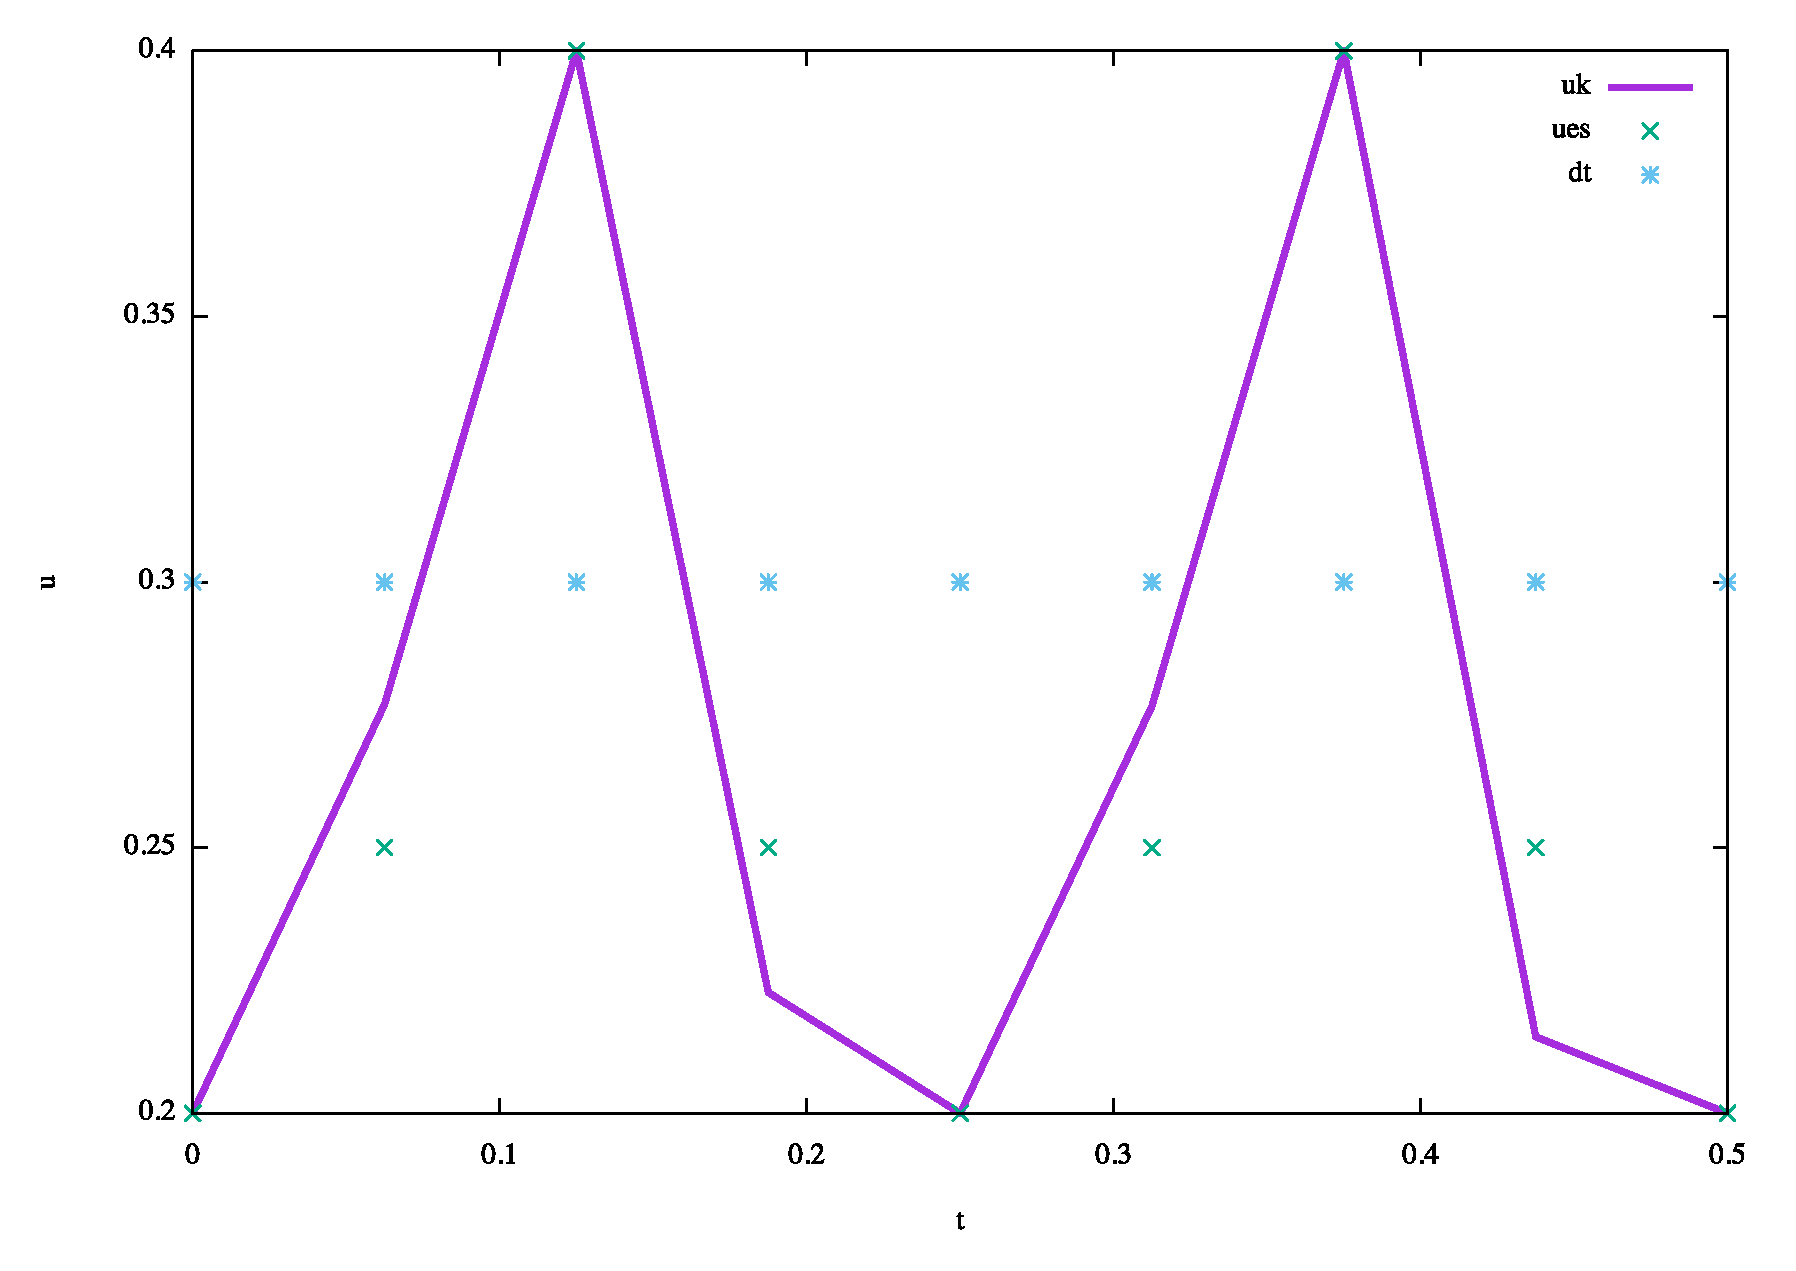
\includegraphics[width=0.3\linewidth]{img/cap6/Imm_PF_02/ControlSol_N150_l3}}\qquad
\subfigure[\protect\url{l = 4}]%
{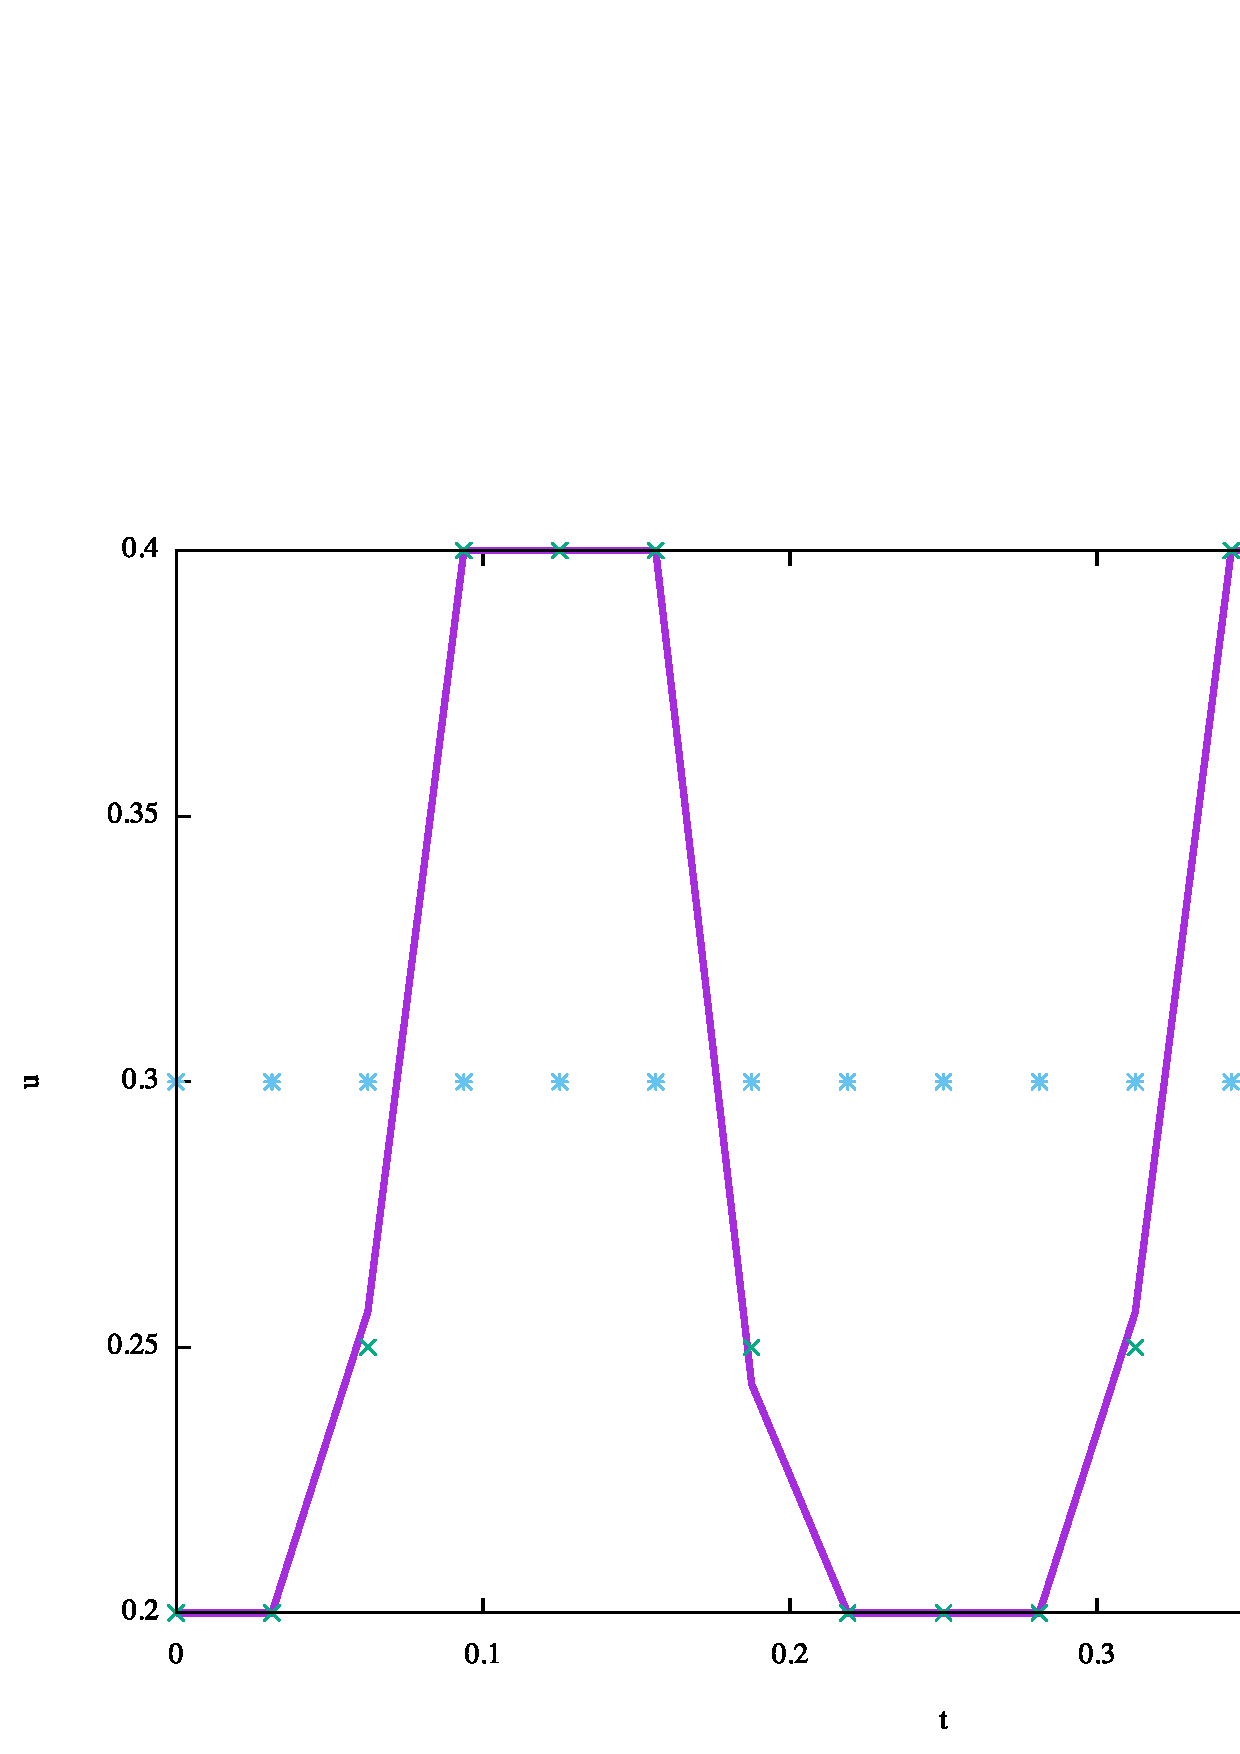
\includegraphics[width=0.3\linewidth]{img/cap6/Imm_PF_02/ControlSol_N150_l4}}\qquad
\subfigure[\protect\url{l = 5}]%
{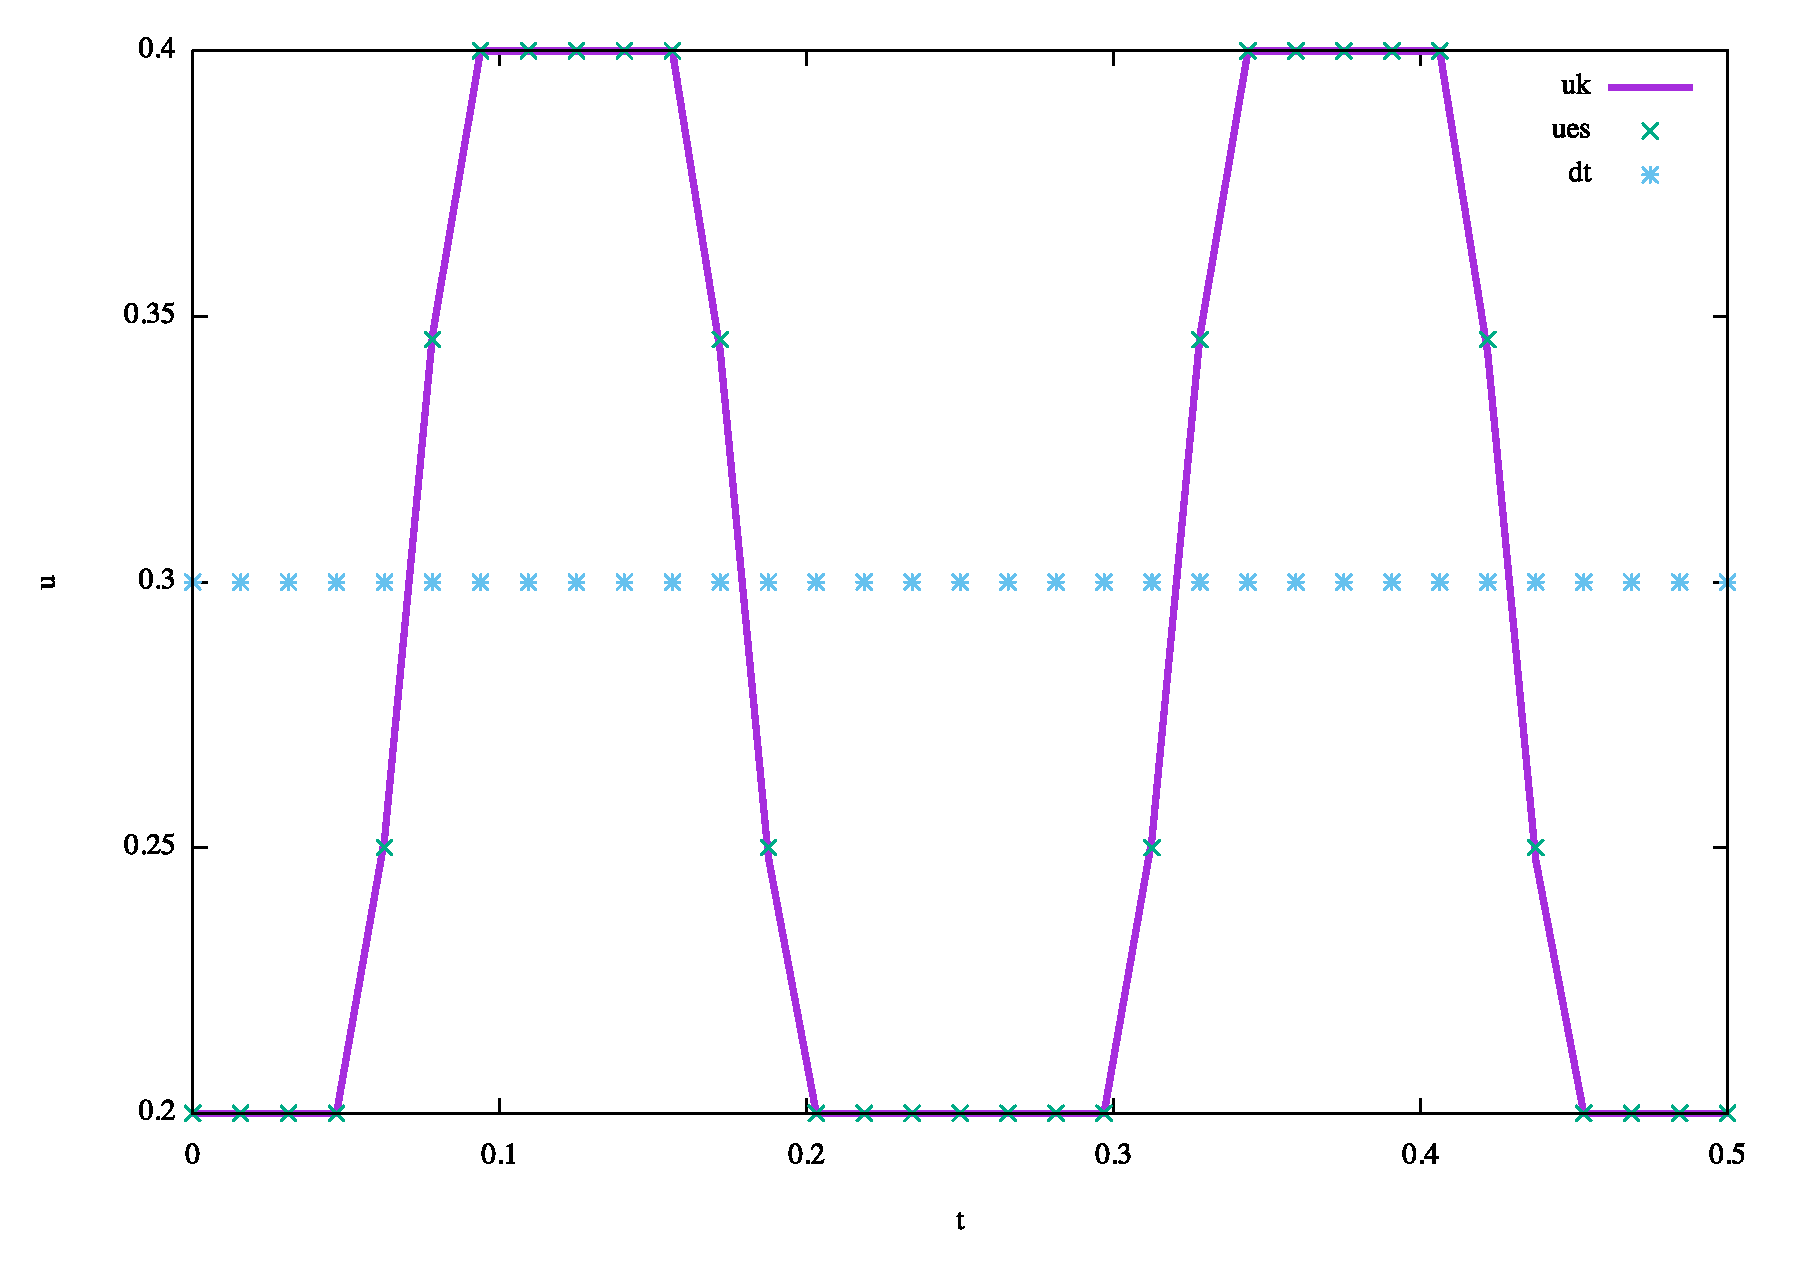
\includegraphics[width=0.3\linewidth]{img/cap6/Imm_PF_02/ControlSol_N150_l5}}\qquad
\subfigure[\protect\url{l = 6}]%
{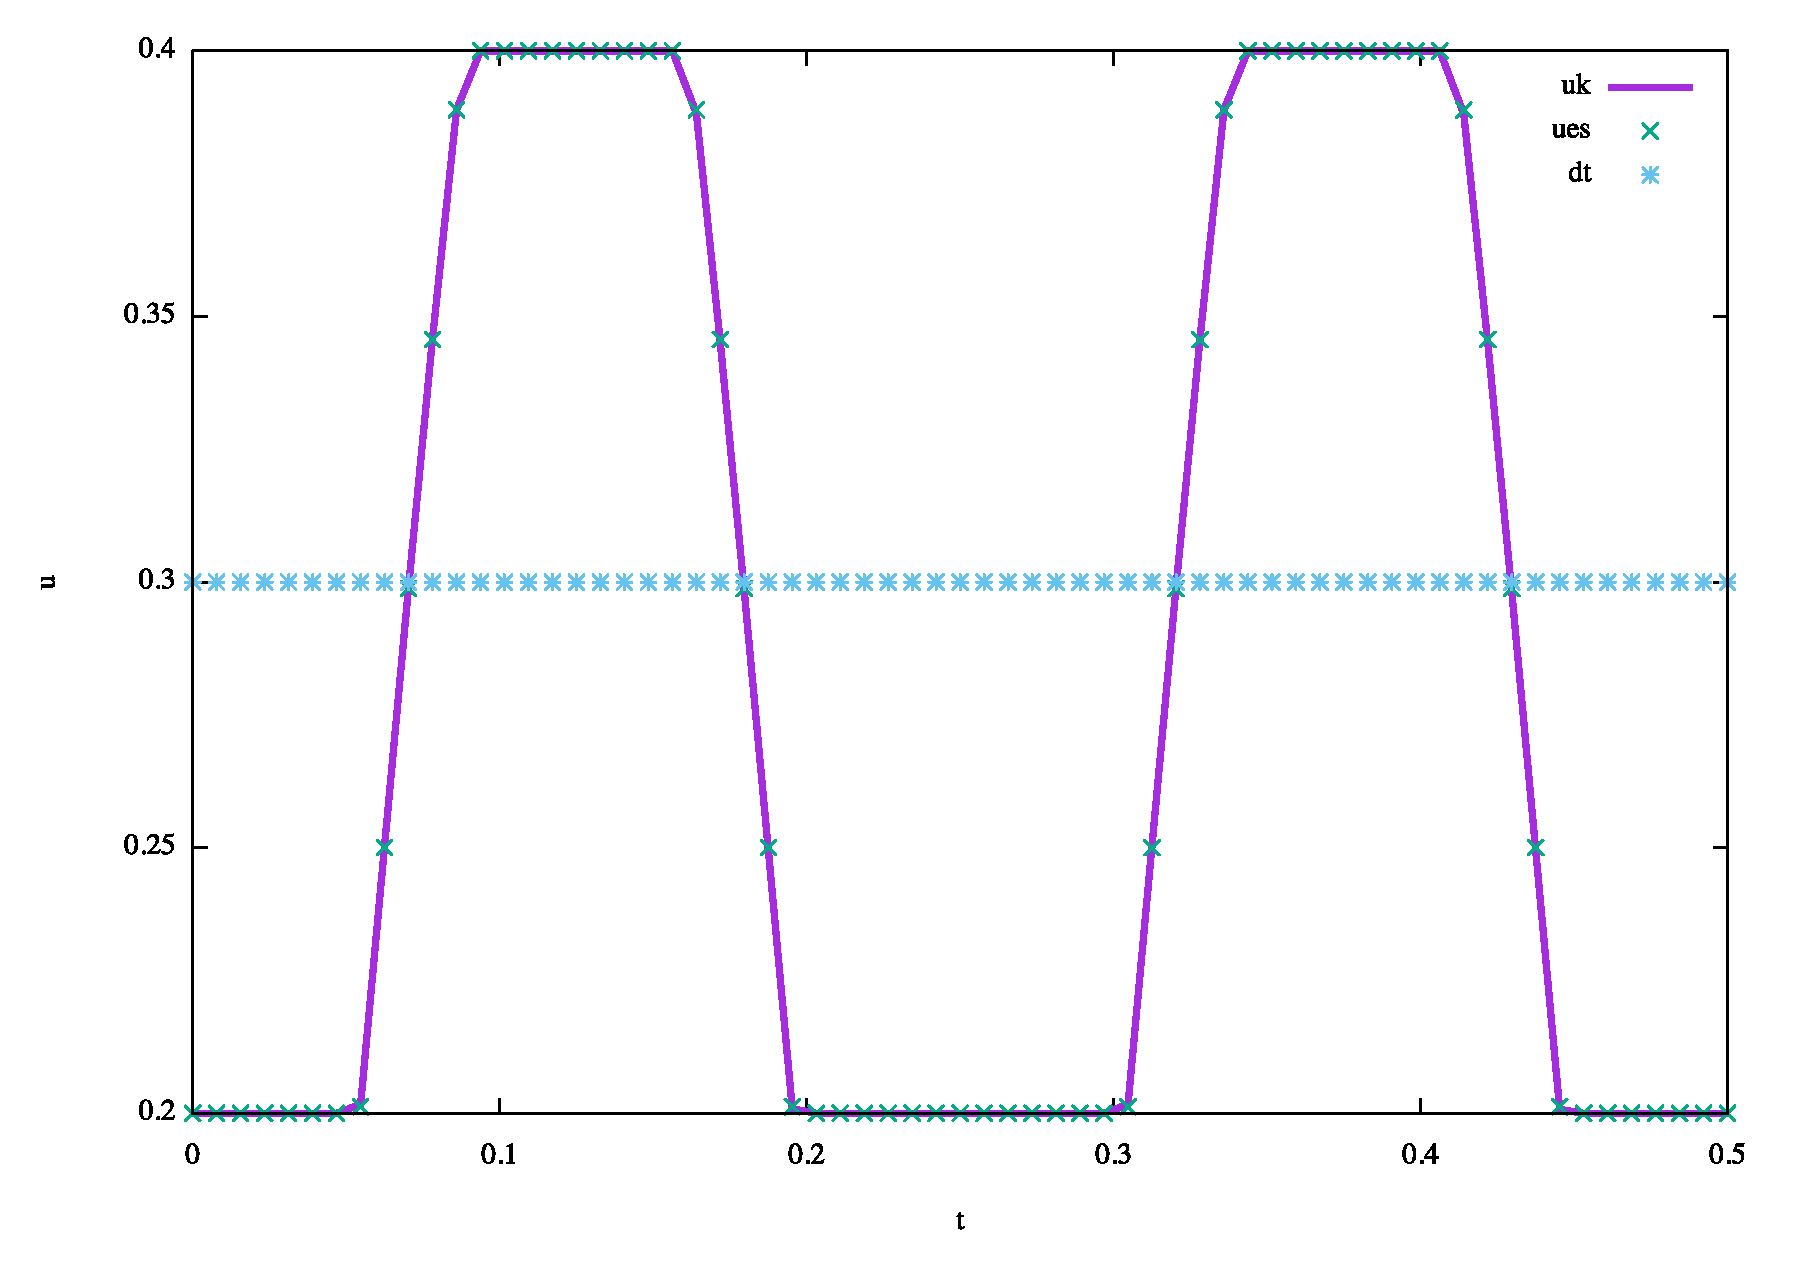
\includegraphics[width=0.3\linewidth]{img/cap6/Imm_PF_02/ControlSol_N150_l6}}\qquad
\subfigure[\protect\url{l = 7}]%
{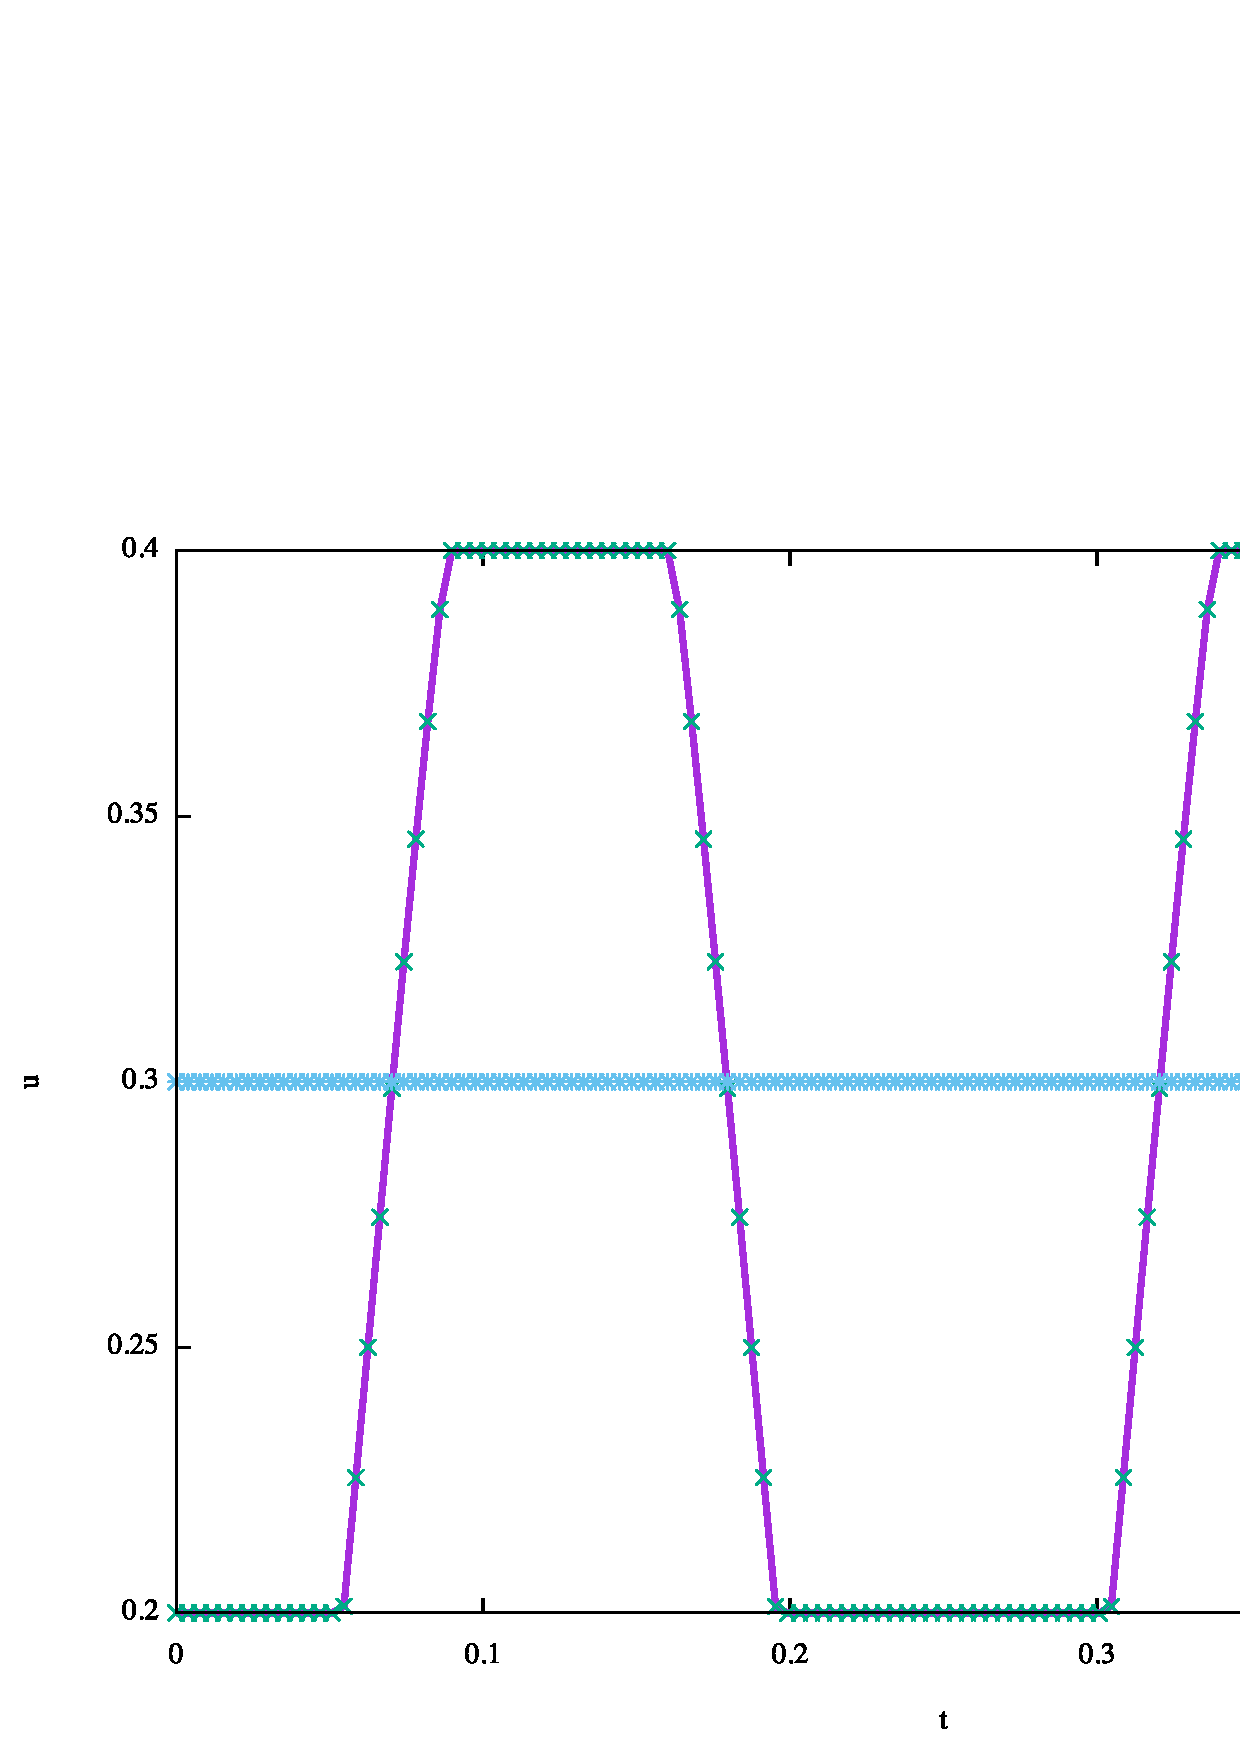
\includegraphics[width=0.3\linewidth]{img/cap6/Imm_PF_02/ControlSol_N150_l7}}\qquad
\subfigure[\protect\url{l = 8}]%
{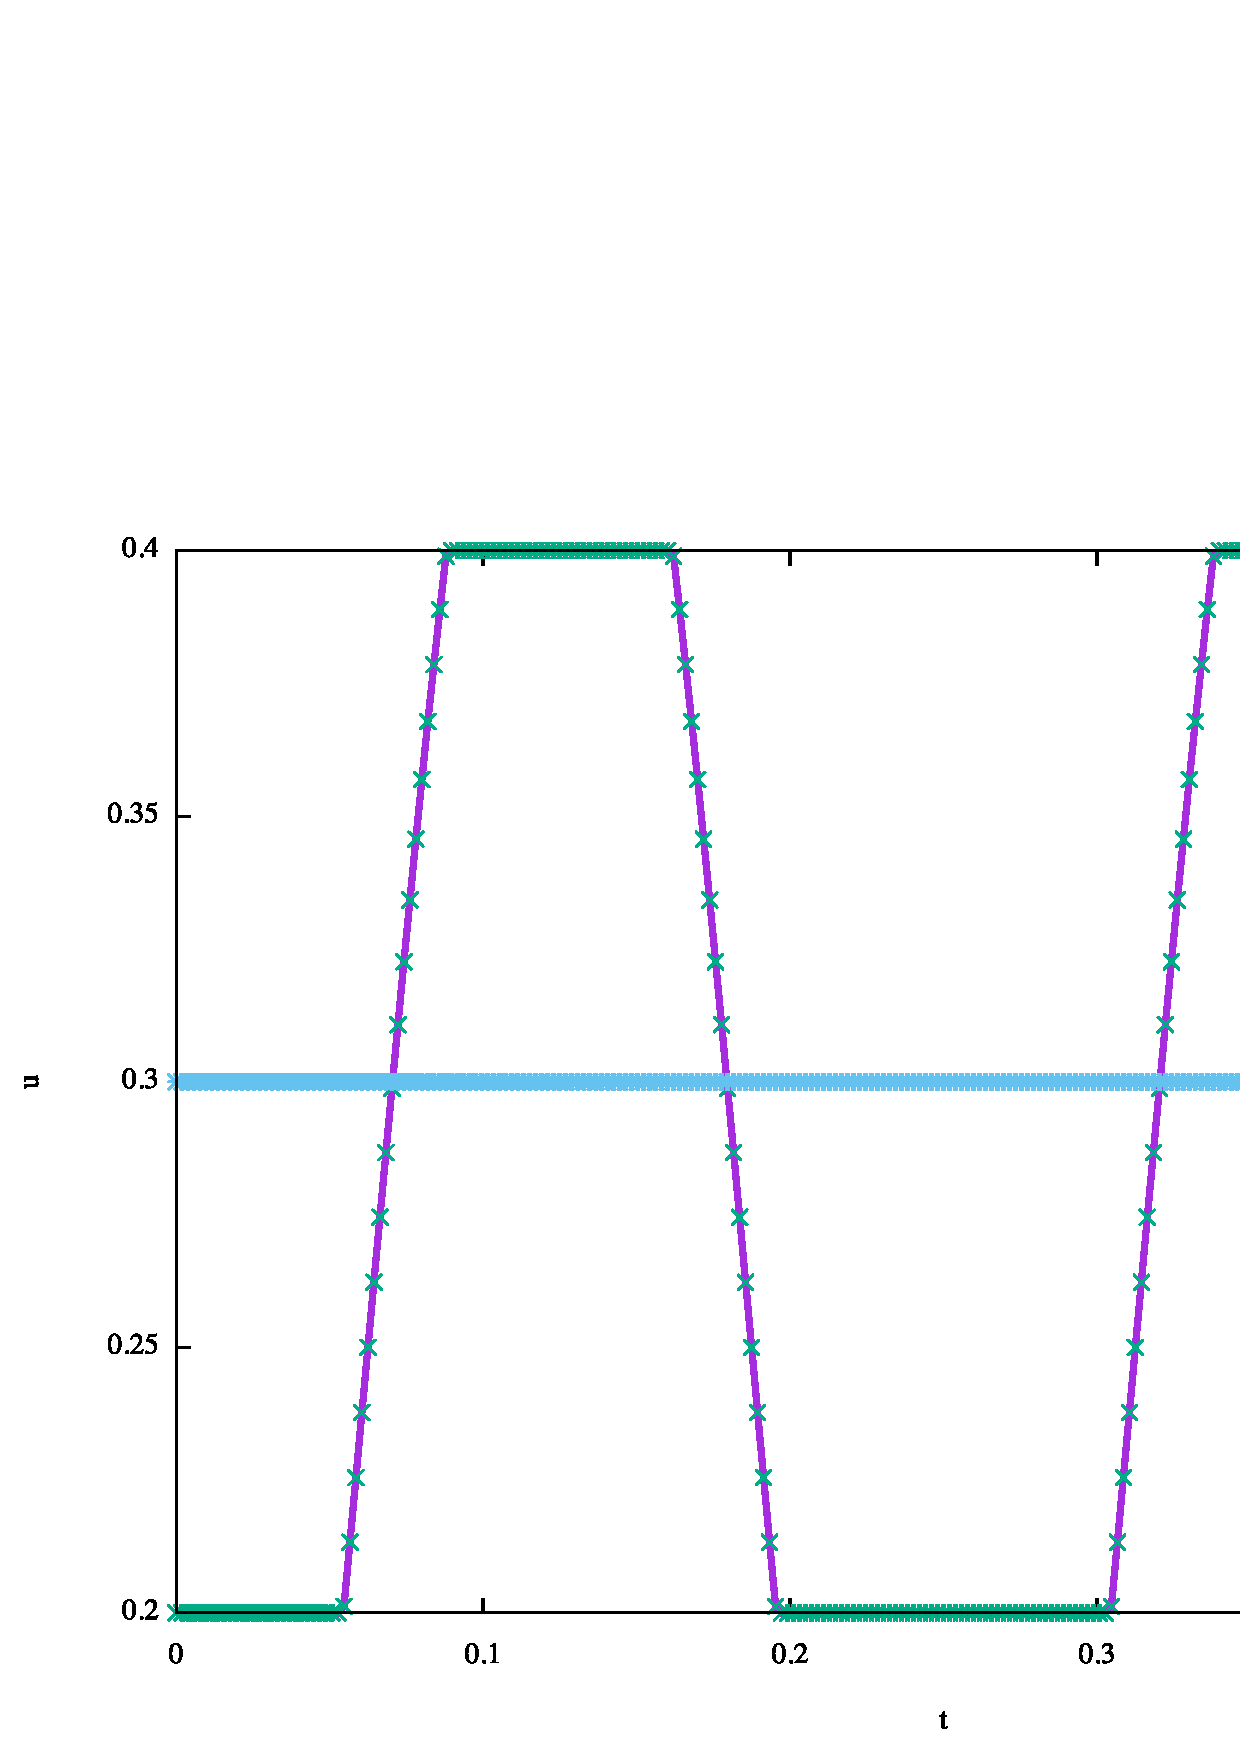
\includegraphics[width=0.3\linewidth]{img/cap6/Imm_PF_02/ControlSol_N150_l8}}
\caption{Test Case 02 $\overline{u}$ e $u_k$ risultati dell'algoritmo di punto fisso}
\label{fig:504}
\end{figure}

\begin{table}
\caption{Newton per Test case II: errori e EOC }
\label{newtonII}
\centering

\begin{tabular}{cllll}
\toprule
{l} &  {$ \norma{\bar{u}-u_{kh}}_{L^2(L^2)} $} &  {$ \norma{\bar{y}-y_{kh}}_{L^2(L^2)} $} &  {$ EOC_{u} $} &  {$ EOC_y $} \\
\midrule
1            &  0.115495 &  0.579976 &  {$-$} &  {$-$} \\
2            &  0.076157  &  0.462076 &  0.815213 &  0.444884 \\
3            &  0.0127336  &  0.136402 &  3.04286 &  2.07579 \\
4            &  0.00222359 &  0.0594457 &  2.74395 &  1.30591 \\
5            &  0.000541362 &  0.0286803 &  2.12996 &  1.09884 \\
6            &  0.000138463  &  0.0142117 &  2.01139 &  1.03579 \\
7            &  0.0000349821 &  0.0070899 &  2.00717 &  1.01455 \\      
8            &  0.0000178053 &  0.003543 &  0.979797  &  1.00643 \\
\bottomrule
\end{tabular}              

\end{table}




\begin{table}
\caption{Newton per Test case II: errori e EOC }
\label{newtonIIbis}
\centering

\begin{tabular}{cllll}
\toprule
{l}  &  {$ \norma{\bar{y}-\pi_{P^*_k}y_{kh}}_{L^2(L^2)} $}  &  {$ \norma{\bar{p}-p_{kh}}_{L^2(L^2)} $}        &  {$ EOC_{\pi y} $} &  {$ EOC_p $} \\
\midrule
1 			 &  0.410488 &  0.57748 &  {$-$} & {$-$} \\
2            &  0.427682 &  0.181205 &  0.080328 &  2.26897 \\
3            &  0.108041 &  0.0846824 &  2.34076 &  1.29421 \\
4            &  0.0223131  &  0.0224907 &  2.48014 &  2.08463 \\
5            &  0.00443687 &  0.00571824 &  2.43516  &  2.06461 \\
6            &  0.0009289  &  0.00145285 &  2.30675 &  2.02121 \\
7            &  0.000203852 &  0.000385873 &  2.21265 &  1.93423 \\      
8            &  0.0000465544 &  0.000130118 &  2.14254 &  1.57714 \\
\bottomrule
\end{tabular}              

\end{table}

\begin{figure}
\centering%
\subfigure[\protect\url{l = 1}]%
{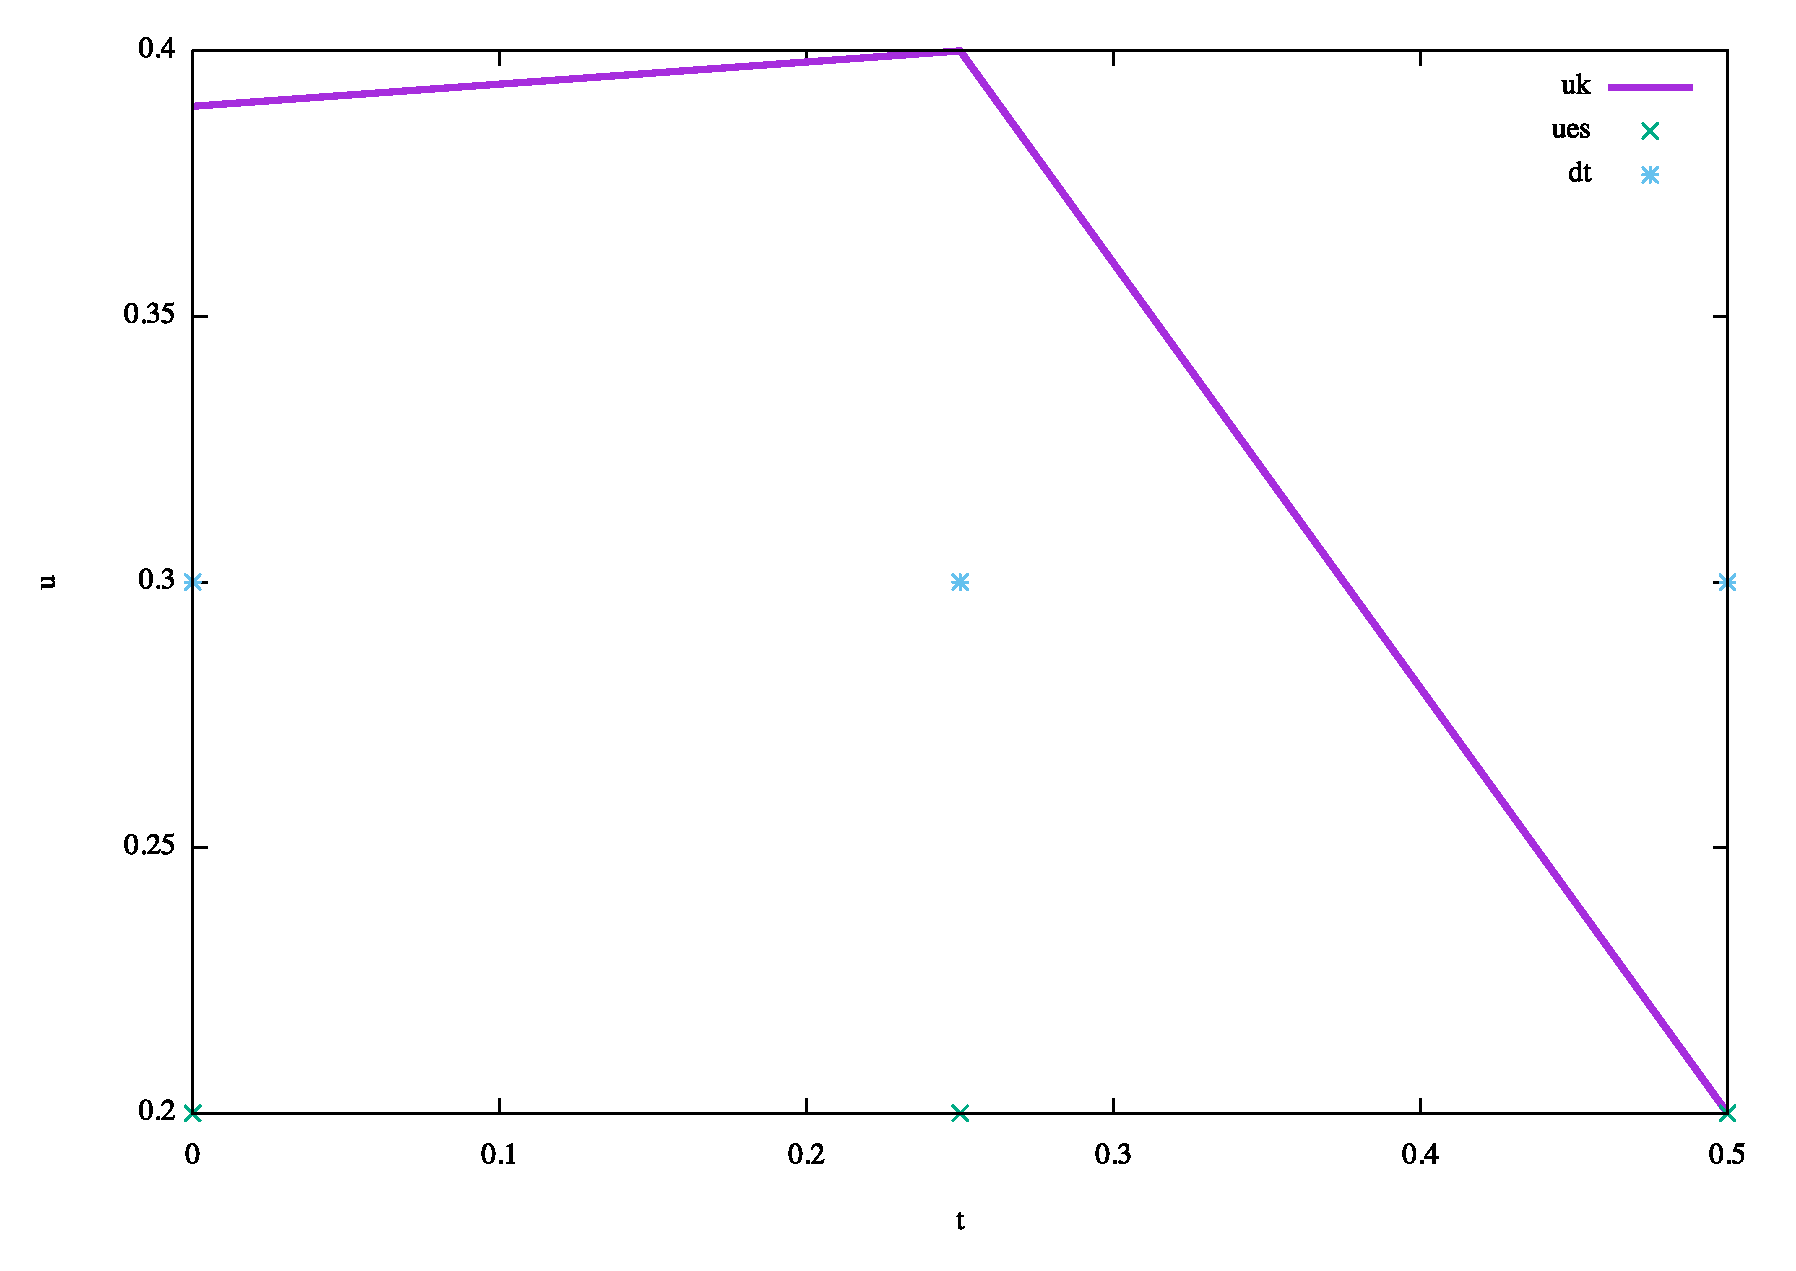
\includegraphics[width=0.3\linewidth]{img/cap6/Imm_CG_02/ControlSol_N150_l1}}\qquad
\subfigure[\protect\url{l = 2}]%
{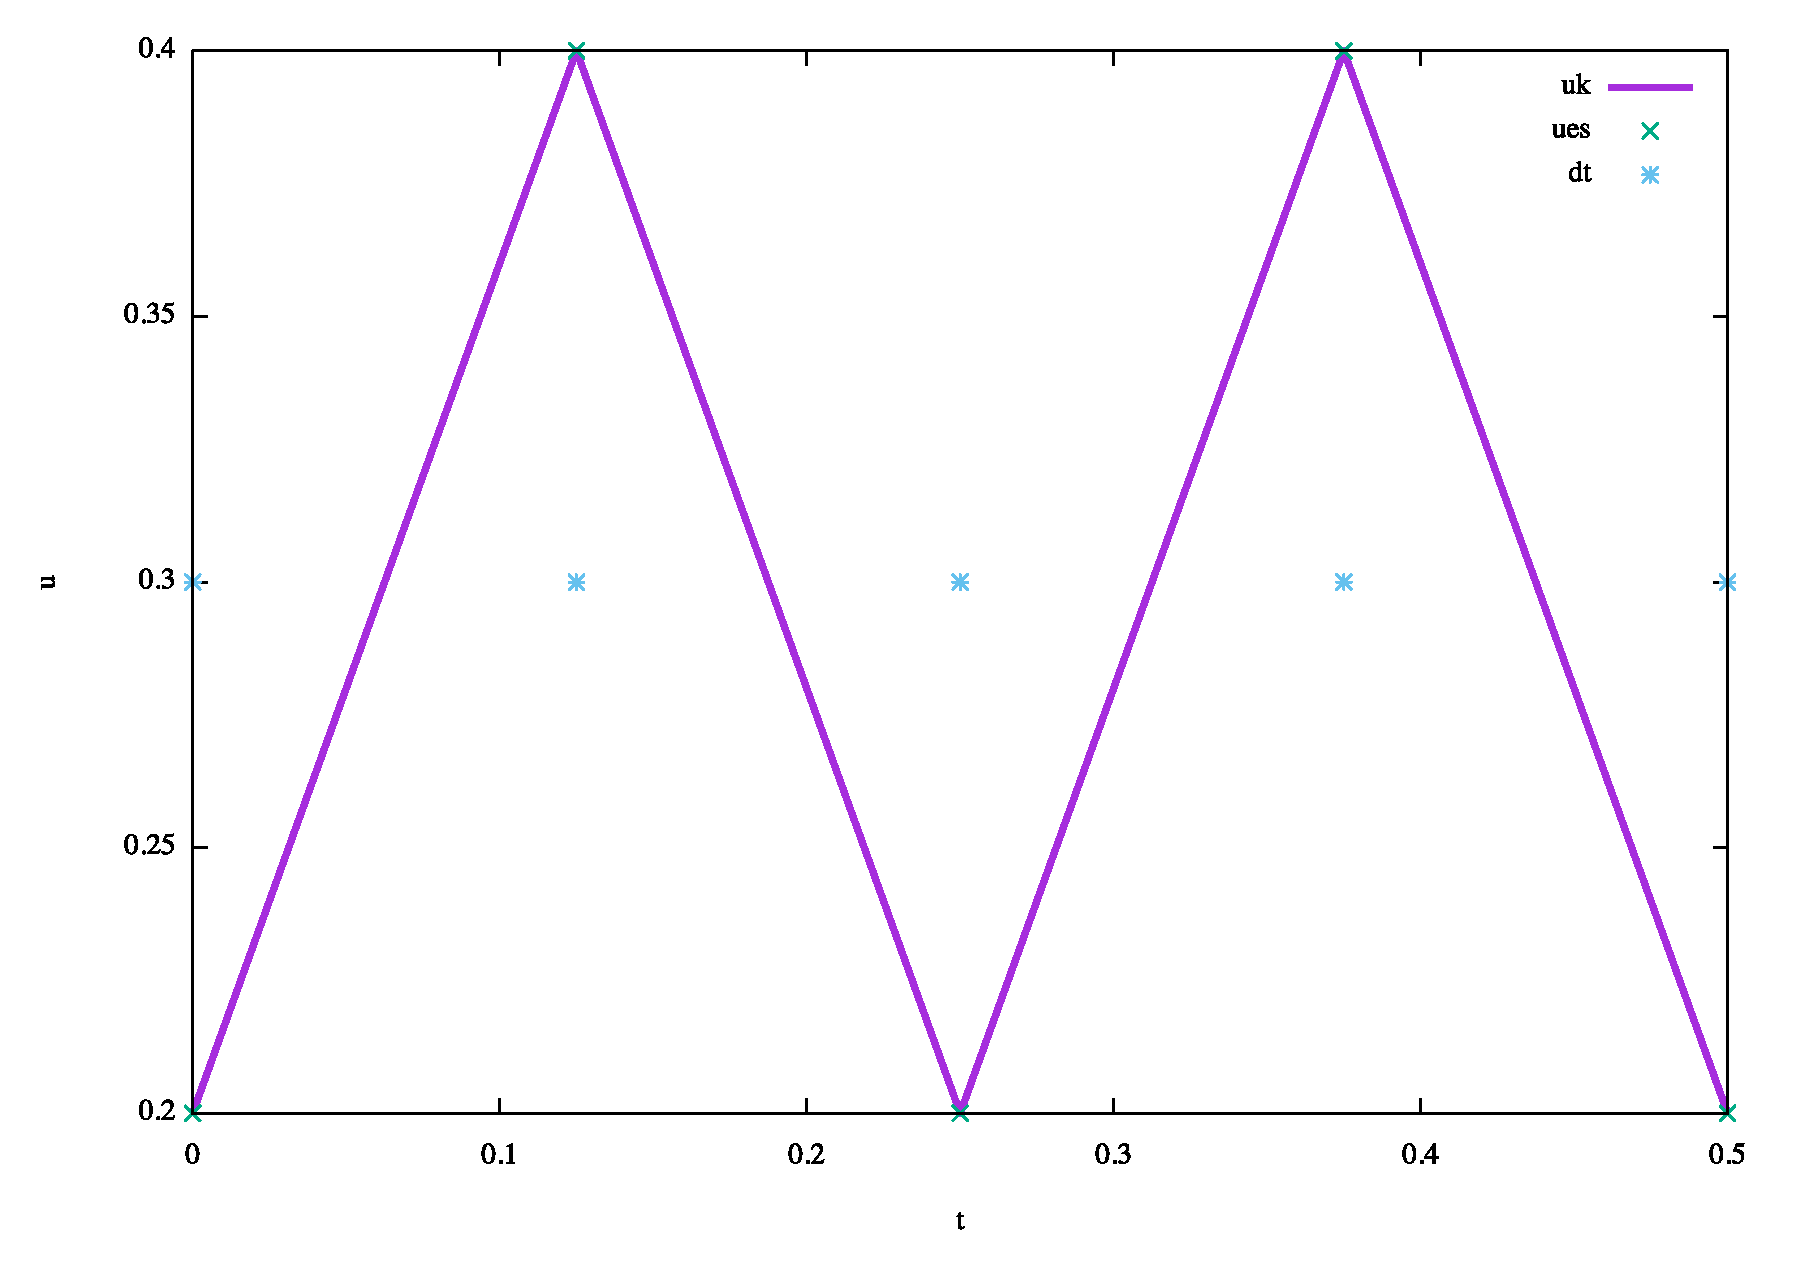
\includegraphics[width=0.3\linewidth]{img/cap6/Imm_CG_02/ControlSol_N150_l2}}\qquad
\subfigure[\protect\url{l = 3}]%
{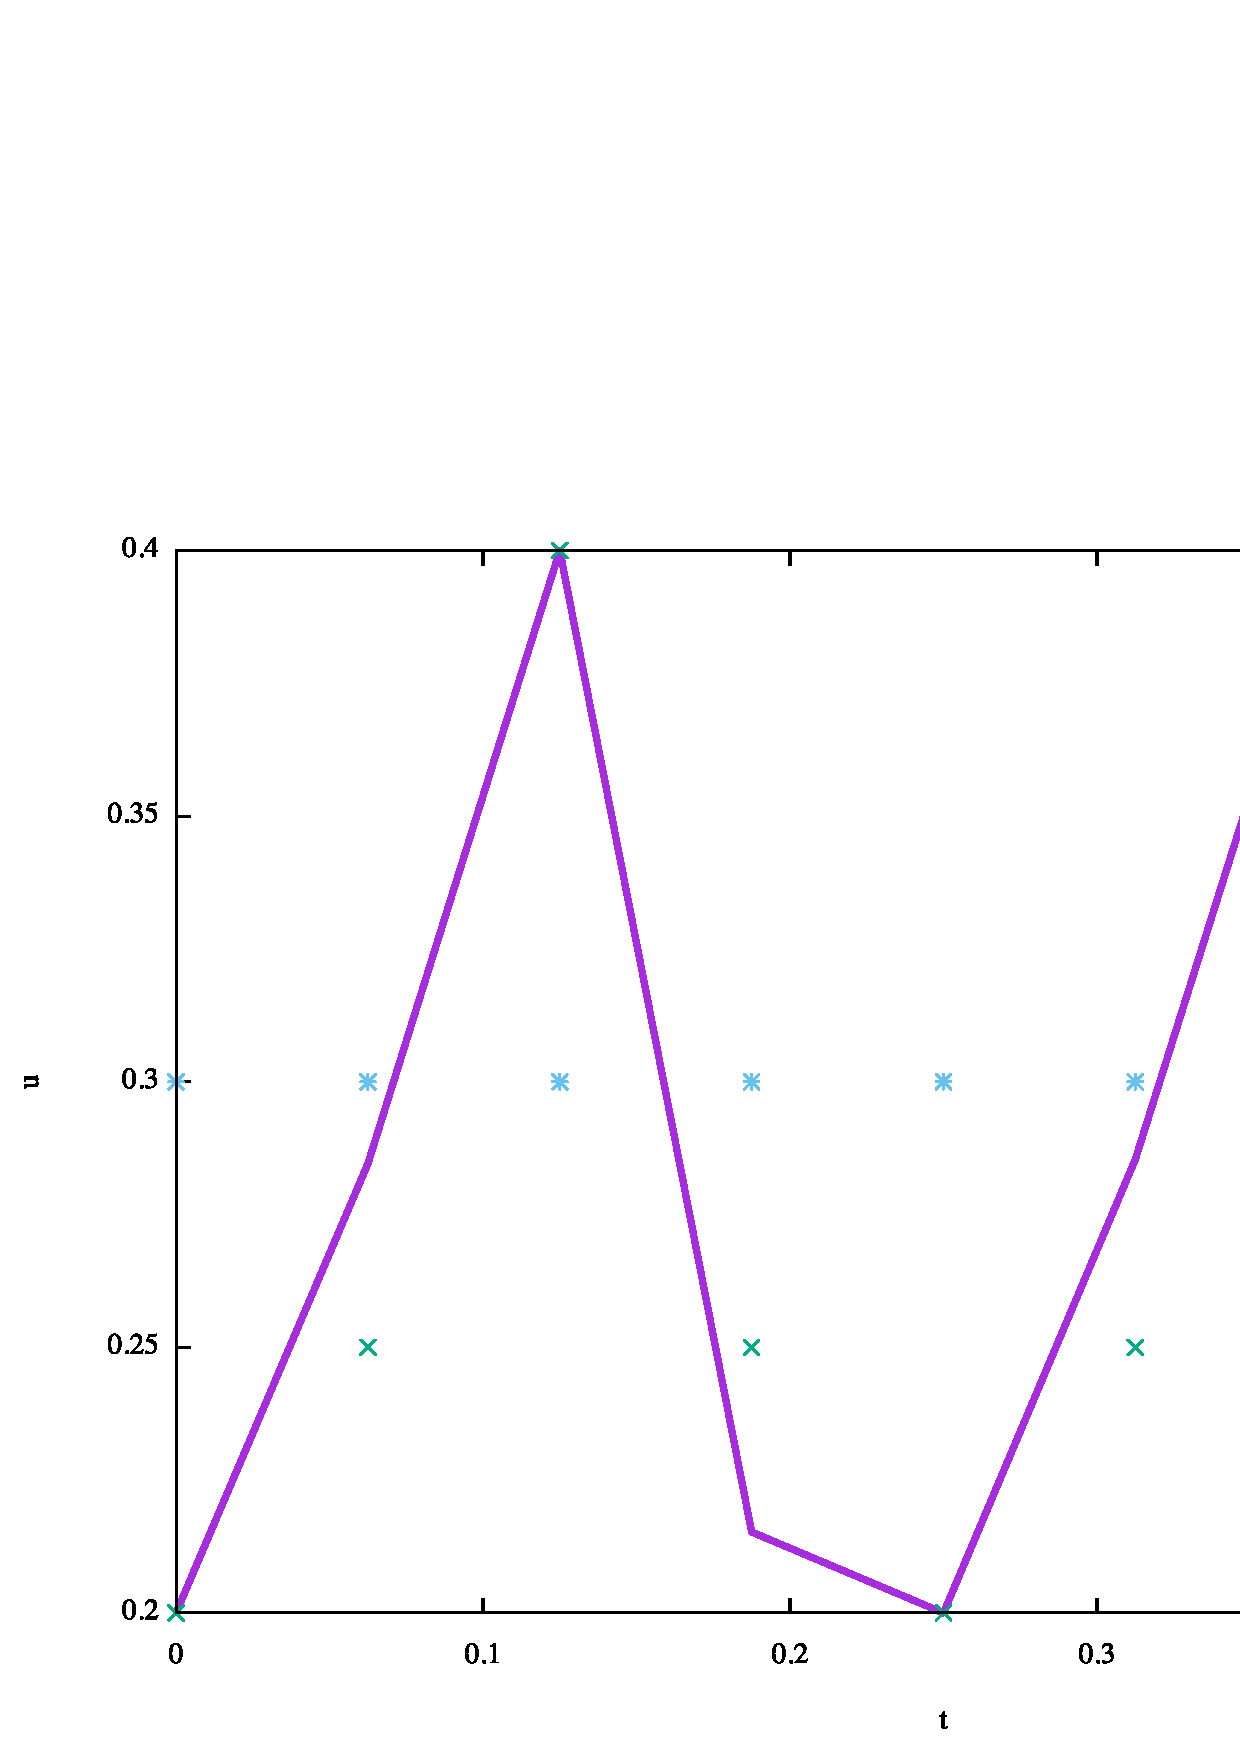
\includegraphics[width=0.3\linewidth]{img/cap6/Imm_CG_02/ControlSol_N150_l3}}\qquad
\subfigure[\protect\url{l = 4}]%
{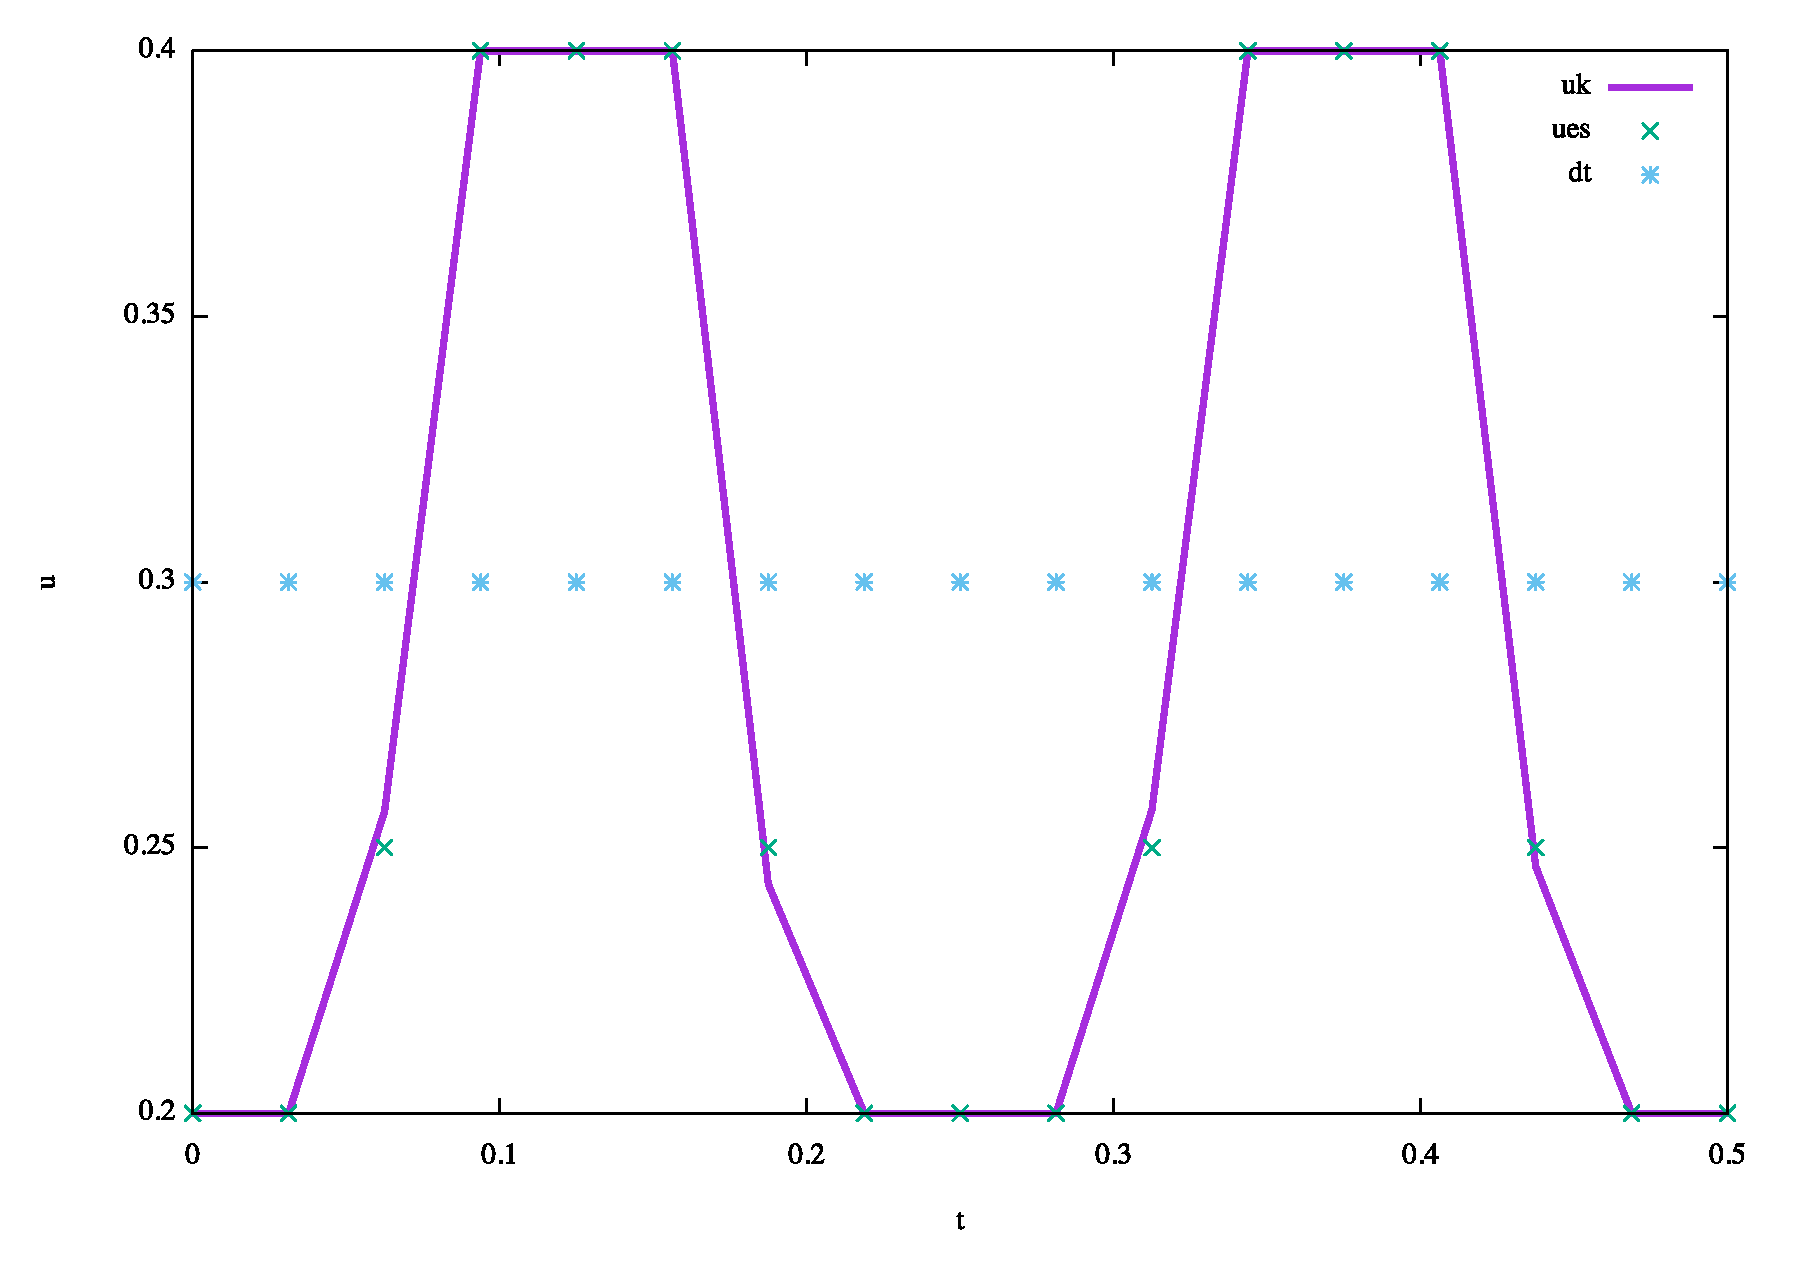
\includegraphics[width=0.3\linewidth]{img/cap6/Imm_CG_02/ControlSol_N150_l4}}\qquad
\subfigure[\protect\url{l = 5}]%
{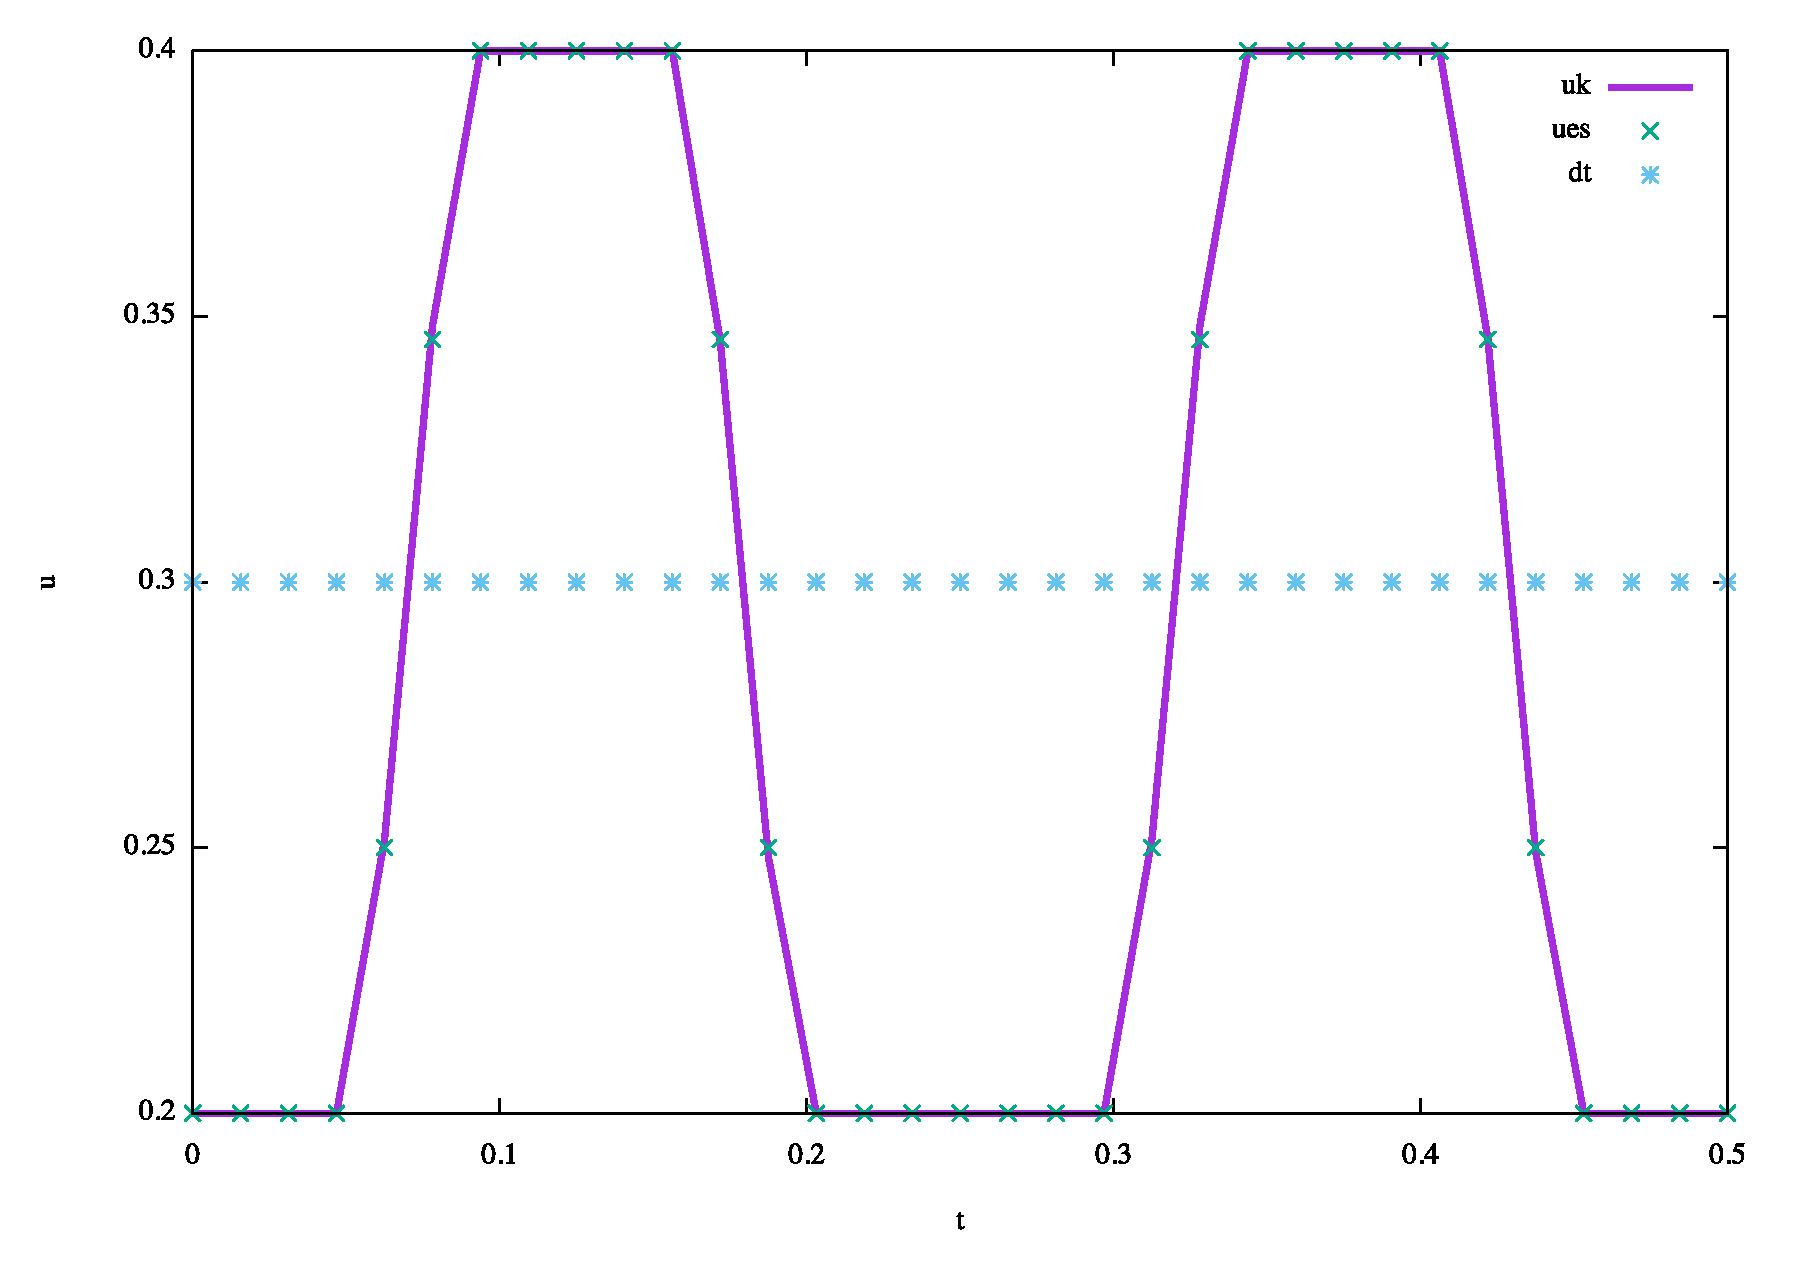
\includegraphics[width=0.3\linewidth]{img/cap6/Imm_CG_02/ControlSol_N150_l5}}\qquad
\subfigure[\protect\url{l = 6}]%
{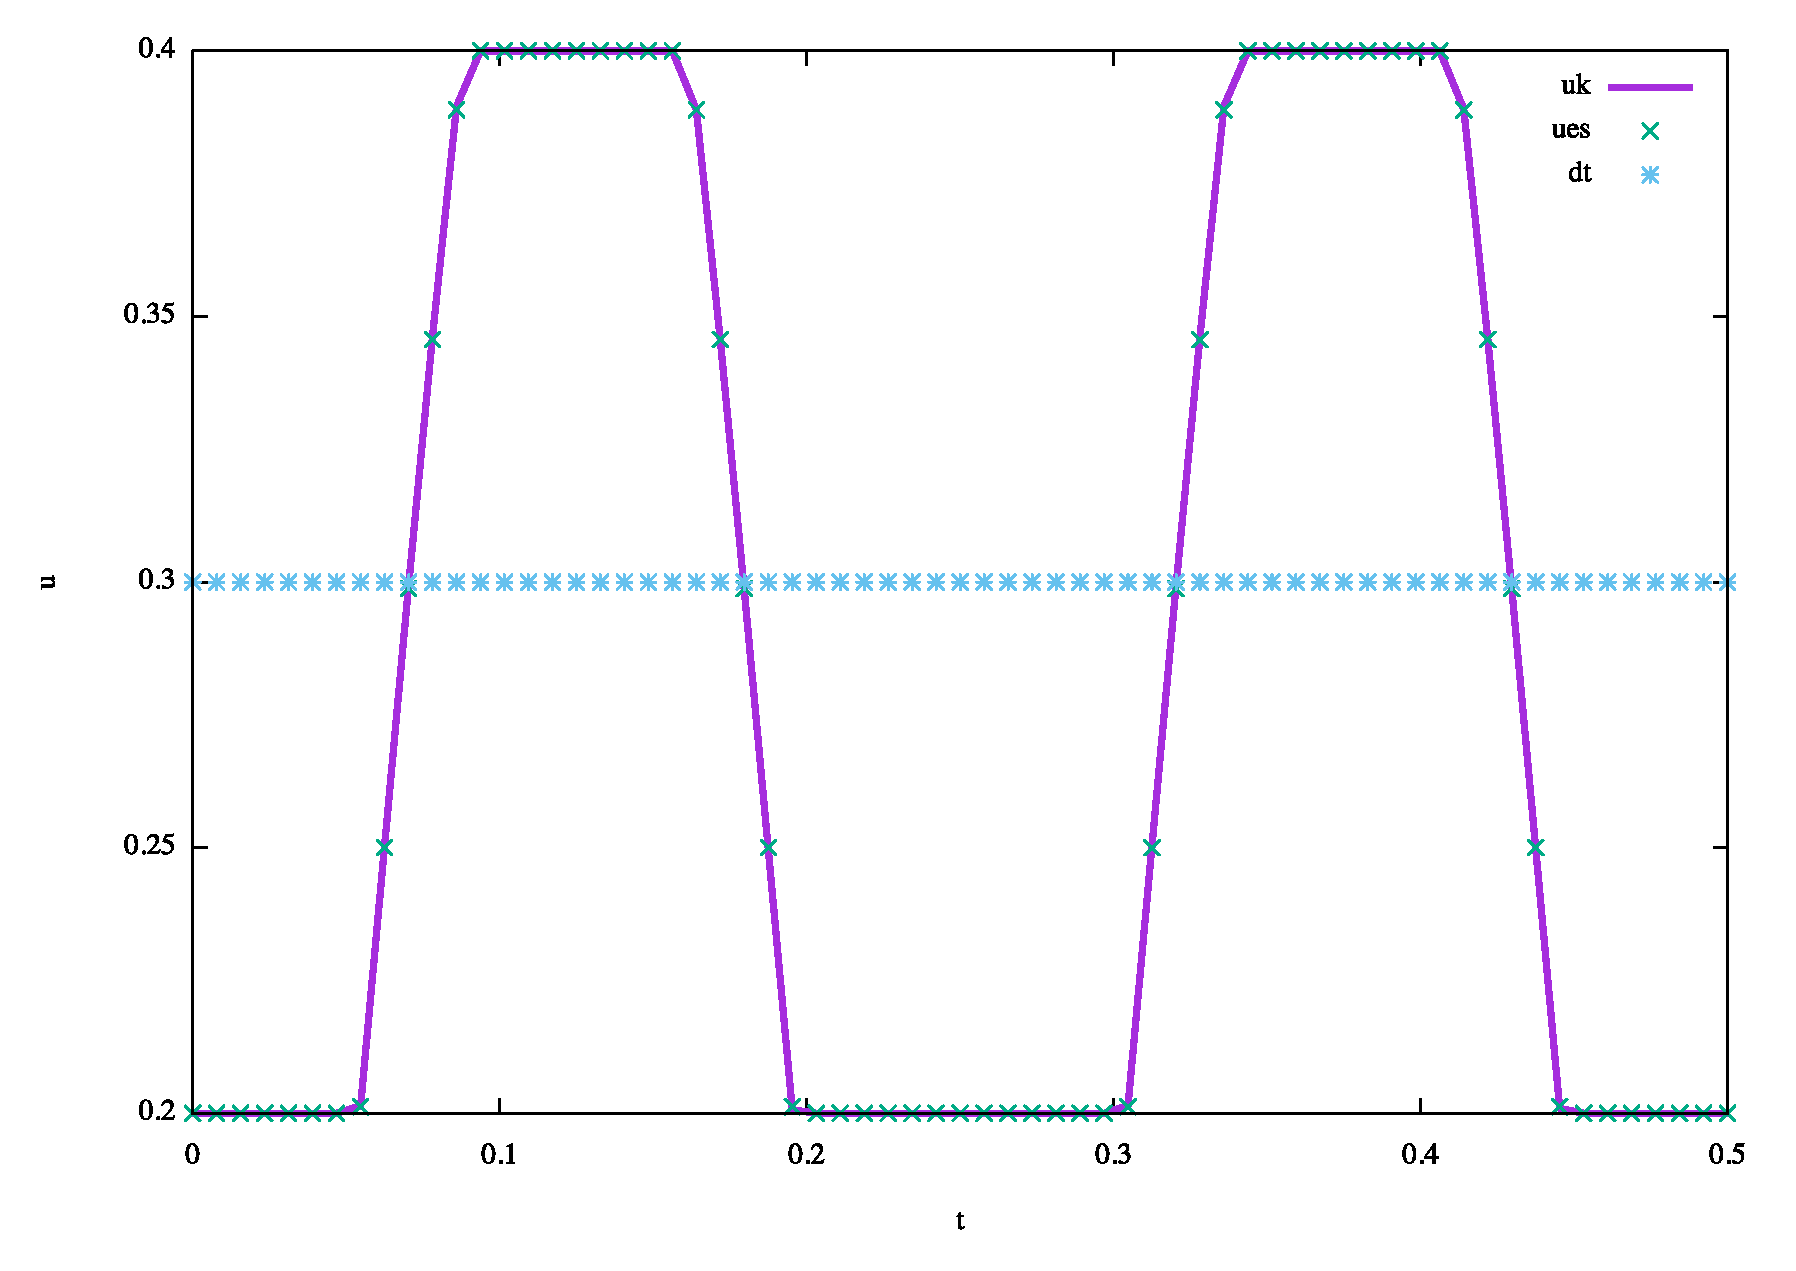
\includegraphics[width=0.3\linewidth]{img/cap6/Imm_CG_02/ControlSol_N150_l6}}\qquad
\subfigure[\protect\url{l = 7}]%
{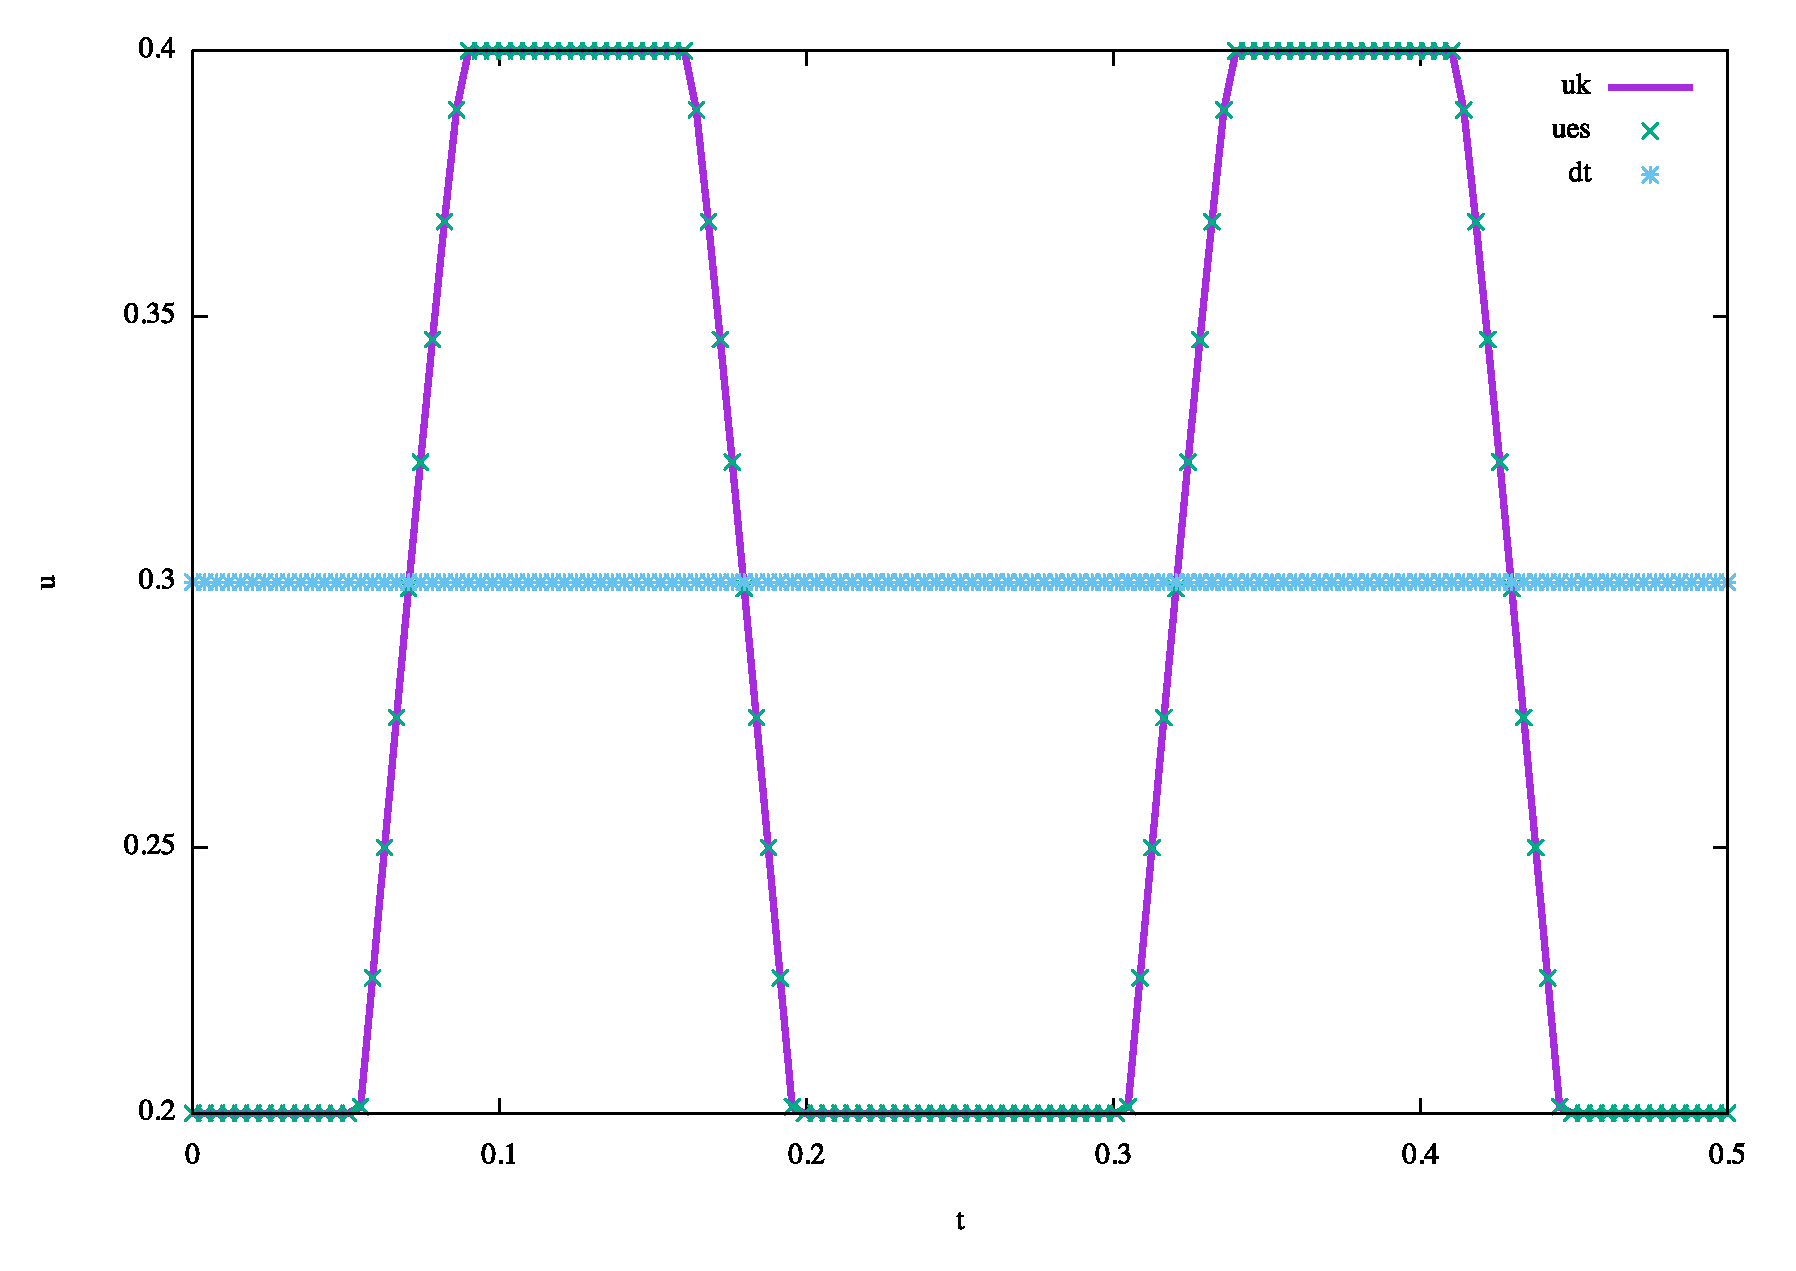
\includegraphics[width=0.3\linewidth]{img/cap6/Imm_CG_02/ControlSol_N150_l7}}\qquad
\subfigure[\protect\url{l = 8}]%
{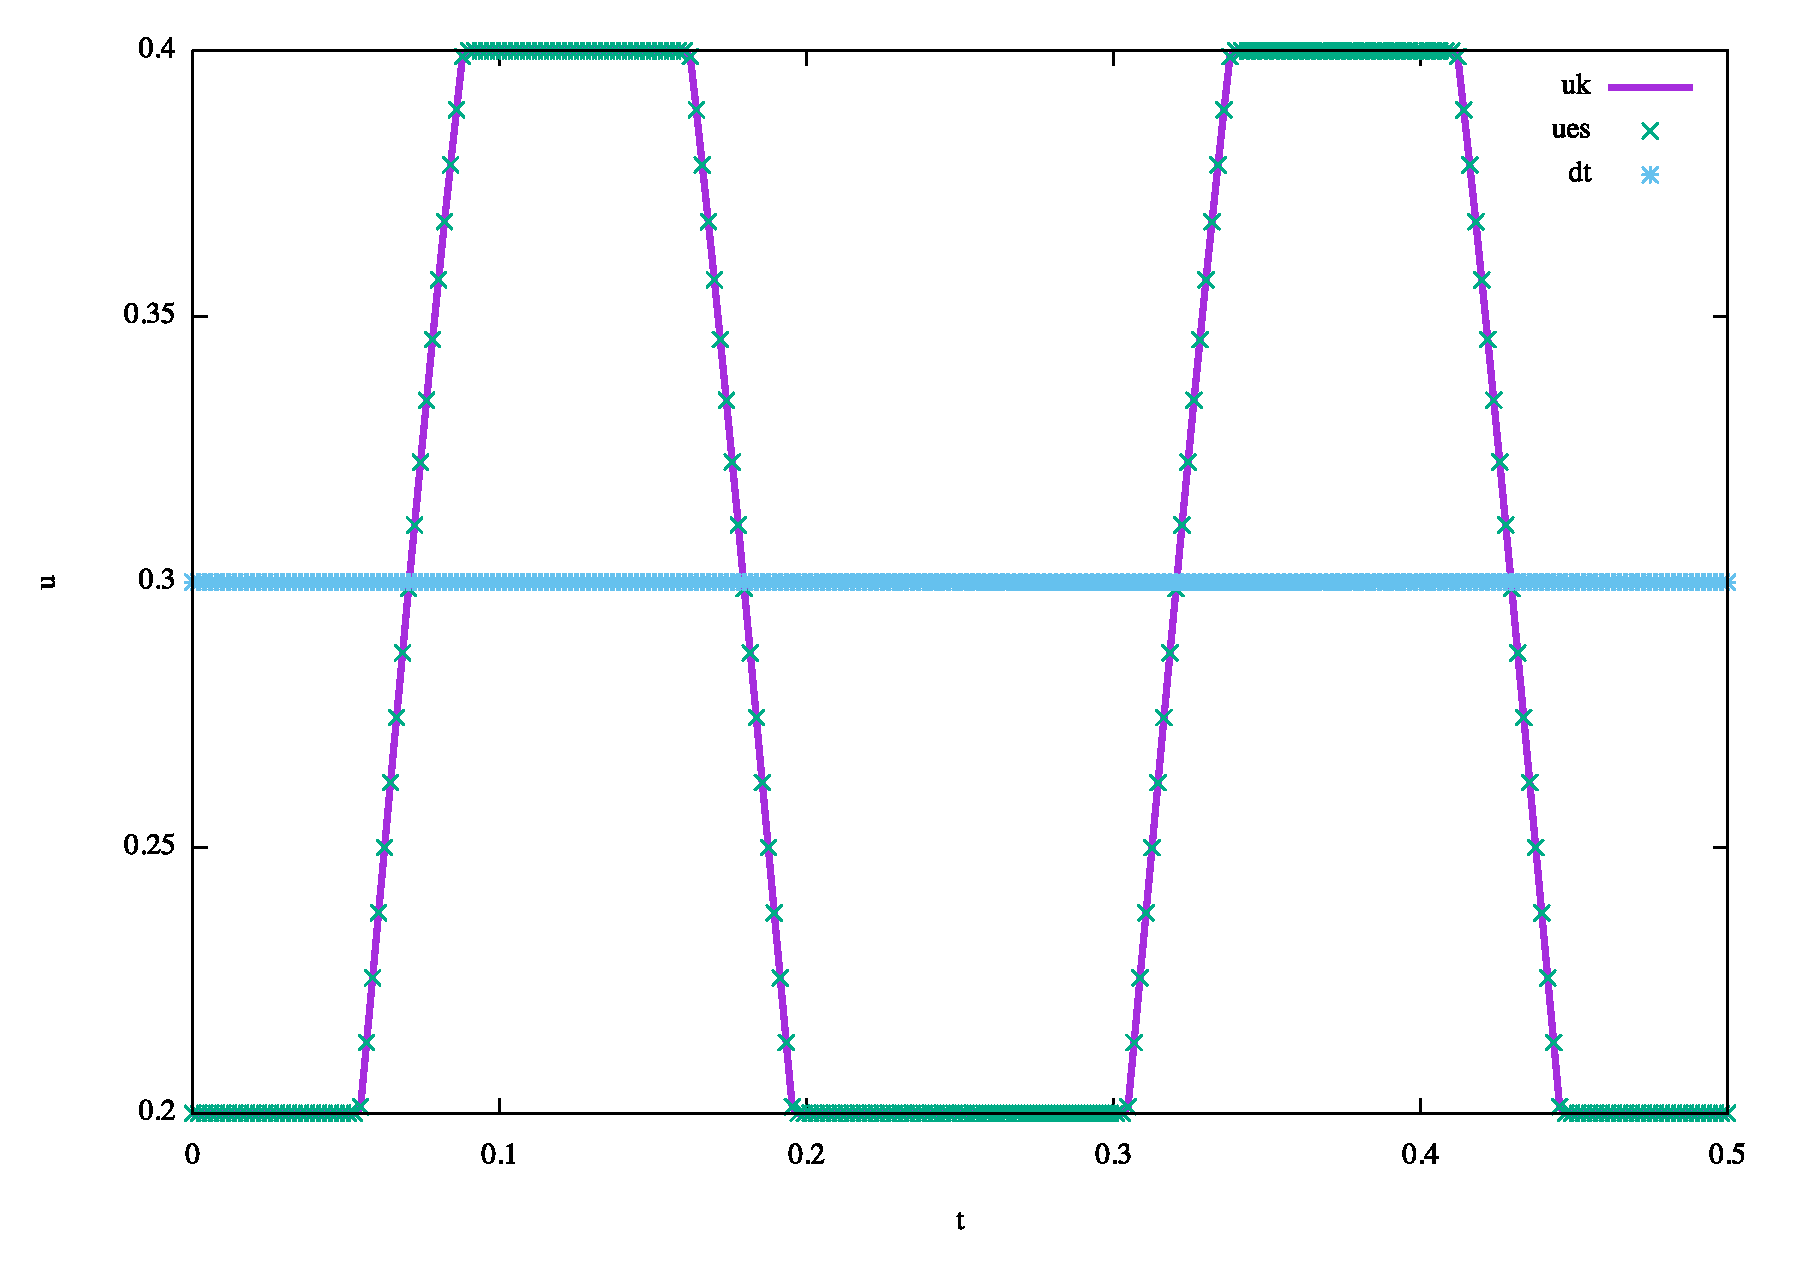
\includegraphics[width=0.3\linewidth]{img/cap6/Imm_CG_02/ControlSol_N150_l8}}
\caption{Test Case 02 $\overline{u}$ e $u_k$: risultati dell'algortimod di semi newton}
\label{fig:505}
\end{figure}